

\documentclass[10pt,journal,compsoc]{IEEEtran}

\usepackage{algorithm}
\usepackage{algorithmic}
\usepackage{amssymb}
\usepackage{amsmath}
\usepackage{color}
\usepackage{graphicx}
\usepackage{subfigure}


\hyphenation{op-tical net-works semi-conduc-tor}


\begin{document}
%\title{Adaptive Partition Testing}
%
%\author{Chang-ai Sun,~\IEEEmembership{Senior Member,~IEEE,}
%        Hepeng Dai,
%        Huai Liu,~\IEEEmembership{Member,~IEEE,}
%        Tsong~Yueh~Chen,~\IEEEmembership{Member,~IEEE},
%        and~Kai-Yuan Cai
%\thanks{C.-A. Sun and H. Dai are with the School of Computer and Communication Engineering, University of Science and Technology Beijing, Beijing 100083, China. E-mail: casun@ustb.edu.cn.}
%\thanks{H. Liu is with the College of Engineering and Science, Victoria University, Melbourne VIC 8001, Australia. E-mail: Huai.Liu@vu.edu.au.}
%\thanks{T.Y. Chen is with the Department of Computer Science and Software Engineering, Swinburne University of Technology, Hawthorn VIC 3122, Australia. Email: tychen@swin.edu.au.}
%\thanks{K.-Y. Cai is with the School of Automation Science and Electrical Engineering, Beihang University, Beijing 100191, China. E-mail: kycai@buaa.edu.cn}}
%
%\markboth{IEEE TRANSACTIONS ON COMPUTERS,~submitted}%
%{Sun \MakeLowercase{\textit{et al.}}: Adaptive Partition Testing}
%
%
%\IEEEtitleabstractindextext{%
%\begin{abstract}
%Random testing and partition testing are two major families of software testing techniques. They have been compared both theoretically and empirically in numerous studies for decades, and it has been widely acknowledged that they have their own advantages and disadvantages and that their innate characteristics are fairly complementary to each other.
%%objective
%Some work has been conducted to develop advanced testing techniques through the integration of random testing and partition testing, attempting to preserve the advantages of both while minimizing their disadvantages. In this paper, we propose a new testing approach,
%\textsl{adaptive partition testing},
%where test cases are randomly selected from some partition whose probability of being selected is adaptively adjusted along the testing process.
%%where test cases are randomly selected from some partitions according to a probability distribution that is adaptively adjusted along the testing process.
%%method
%We particularly develop two algorithms,
%%\textsl{Markov-chain adaptive partition testing} and \textsl{reward-punishment adaptive partition testing}, to implement the new approach. The former algorithm makes use of Markov matrix to dynamically adjust the probability of a partition to be selected for generating test cases;
%\textsl{Markov-chain based adaptive partition testing} and \textsl{reward-punishment based adaptive partition testing}, to implement the proposed  approach. The former algorithm makes use of Markov matrix to dynamically adjust the probability of a partition to be selected for conducting tests;
%while the latter is based on the reward and punishment mechanism.
%%results
%We conduct empirical studies to evaluate the performance of the proposed algorithms using ten faulty versions of three large-scale open source programs.
%%Our experimental results show that both algorithms have high fault-detection effectiveness and low test case selection overhead.
%Our experimental results show that, compared with two baseline techniques, namely Random Partition Testing (RPT) and Dynamic Random Testing (DRT), our algorithms deliver higher fault-detection effectiveness with lower test case selection overhead.
%%conclusion
%It is demonstrated that the proposed adaptive partition testing is an effective testing approach, taking advantages of both random testing and partition testing.
%\end{abstract}
%
%% Note that keywords are not normally used for peerreview papers.
%\begin{IEEEkeywords}
%Random testing, partition testing, adaptive partition testing.
%\end{IEEEkeywords}}
%
%
%% make the title area
%\maketitle
%
%
%% To allow for easy dual compilation without having to reenter the
%% abstract/keywords data, the \IEEEtitleabstractindextext text will
%% not be used in maketitle, but will appear (i.e., to be "transported")
%% here as \IEEEdisplaynontitleabstractindextext when the compsoc
%% or transmag modes are not selected <OR> if conference mode is selected
%% - because all conference papers position the abstract like regular
%% papers do.
%\IEEEdisplaynontitleabstractindextext
%% \IEEEdisplaynontitleabstractindextext has no effect when using
%% compsoc or transmag under a non-conference mode.
%
%
%
%% For peer review papers, you can put extra information on the cover
%% page as needed:
%% \ifCLASSOPTIONpeerreview
%% \begin{center} \bfseries EDICS Category: 3-BBND \end{center}
%% \fi
%%
%% For peerreview papers, this IEEEtran command inserts a page break and
%% creates the second title. It will be ignored for other modes.
%\IEEEpeerreviewmaketitle
%
%
%
%\IEEEraisesectionheading{\section{Introduction}\label{sec:introduction}}
%
%
%\IEEEPARstart{S}{oftware} testing is a major approach to assessing and assuring the reliability of the software under development. In the past few decades, we have seen lots of testing techniques proposed and developed based on different intuitions and for serving various purposes. Among them, random testing (RT)~\cite{Hamlet02} and partition testing (PT)~\cite{Weyuker91} represent two fundamental families of testing techniques.
%
%In RT, test cases are randomly selected from the input domain (which refers to the set of all possible inputs of the software under test). Traditionally, when the testing purpose is to detect software faults, the random test case selection is normally based on the uniform distribution, that is, each possible input has the same probability to be selected as a test case. On the other hand, if the testing purpose is the reliability assessment, RT follows a so-called operational profile, which refers to the probability distribution according to users' normal operations.
%
%Different from RT, PT was originally proposed to generate test cases in a more ``systematic'' way, aiming at improving the effectiveness of fault detection. The input domain is first divided into disjoint partitions, and test cases are then selected from each and every partition. In PT, each partition is expected to have a certain degree of homogeneity, that is, inputs in the same partition should cause similar software execution behavior. In the ideal case, a partition should be homogeneous, that is, if one input is fault-revealing/non-fault-revealing, all other inputs in the same partition will be fault-revealing/non-fault-revealing too.
%
%Since 1980s or even earlier, RT and PT have been compared with each other in terms of their fault detection effectiveness~\cite{Hamlet90, ChenTSE94, ChenTSE96, Gutjahr99}. It had been surprising to quite a few people that PT, considered as more systematic, does not outperform RT too much, and that in some circumstances, RT even has higher effectiveness than PT. Intuitively speaking, PT should be very effective if each partition is homogeneous. However, such a homogeneity cannot be guaranteed in practice, and hence PT may be ineffective. In contrast, RT selects test cases in a random manner, so it is possible that it misses some faults that could easily be revealed by PT; on the other hand, also due to its randomness, RT can sometimes reveal non-trivial faults that are difficult to be detected by PT.
%
%Generally speaking, RT and PT are based on fundamentally different intuitions. Therefore, it is likely that they can be complementary to each other in detecting various types of faults. It is thus interesting to investigate the integration of them for developing new testing techniques. In fact, Cai et al.~\cite{Cai05, Cai07} have proposed the so-called random partition testing (RPT). In RPT, the input domain is first divided into $m$ partitions $c_1, c_2, \ldots, c_m$, and each $c_i$ is allocated a probability $p_i$. A partition $c_i$ is randomly selected according to the testing profile $\{p_1, p_2, \ldots, p_m\}$, where $p_1 + p_2 + \cdots +p_m = 1$. A concrete test case is then randomly selected from the chosen $c_i$.
%
%Independent researchers from various areas have individually observed that the fault-revealing inputs tend to cluster into ``continuous regions''~\cite{Ammann88, Finelli91}. Based on this observation, Cai et al.~\cite{Cai09} further proposed the so-called dynamic random testing (DRT) technique based on the theory of software cybernetics~\cite{Cai02}. Different from the original RPT, where the values of $p_i$ are fixed and kept static along the testing process, DRT attempts to dynamically change the values of $p_i$: If a test case from a partition $c_i$ reveals a fault, the corresponding $p_i$ will be increased by a constant $\epsilon$; otherwise, decreased by another constant $\delta$. Although DRT is more effective than RPT, it also has its own problems, such as an appropriate assignment of values for ($\epsilon$ and $\delta$), and the inefficiency in locating the partitions with higher fault-revealing probability.
%
%%the fixed values ($\epsilon$ and $\delta$) for $p_i$'s adjustment, and the low speed in finding the partitions with higher fault-revealing probability (i.e. the possible assignment of a higher probability to partitions without revealing faults).
%%and the low speed in finding the partitions with high fault-revealing ratios.
%
%In this paper, we propose a new testing approach, namely adaptive partition testing (APT), of integrating RT and PT. The key component of APT is a novel mechanism of adaptively changing the adjustments to $p_i$ along the testing process. The major contributions of our study are as follows.
%
%\begin{itemize}
%	\item We develop two algorithms for APT, namely Markov-chain based APT (MAPT) and reward-punishment based APT (RAPT), which, as their names manifest, implement the adaptive adjustment of $p_i$ based on the Markov matrix and the reward and punishment mechanism, respectively.
%	\item The performance of MAPT and RAPT is evaluated through a series of empirical studies on large-scale open source programs. It is shown that both MAPT and RAPT have significantly higher fault-detection effectiveness than RPT and DRT, while their test case selection overhead is lower.
%\end{itemize}
%
%The rest of the paper is organized as follows. In Section~\ref{sec:approach}, we introduce the basic intuition of APT, and present the algorithms of MAPT and RAPT. In Section~\ref{sec:exp}, we discuss the settings of empirical studies for evaluating MAPT and RAPT, the results of which are summarized in Section~\ref{sec:results}. The previous work closely related to APT is discussed in Section~\ref{sec:related}. Finally, we conclude the paper in Section~\ref{sec:conc}.
%
%\section{Our Approach}
%\label{sec:approach}
%
%\subsection{Intuition}
%
%Let us first look at how DRT adjusts the value of $p_i$. Suppose that a test case from $c_i$ ($i = 1, 2, \ldots, m$) is selected and executed. If this test case reveals a fault, $\forall j = 1, 2, \ldots, m$ and $j \neq i$, we set
%
%\begin{equation}
%\label{eq:DRThitJ}
%%\text{new} p_j =
%p'_j =
%\begin{cases}
%p_j - \displaystyle\frac{\epsilon}{m-1} & \text{if } p_j \geq \displaystyle\frac{\epsilon}{m-1} \\
%0 & \text{if } p_j < \displaystyle\frac{\epsilon}{m-1}
%\end{cases},
%\end{equation}
%
%and then set
%
%\begin{equation}
%\label{eq:DRThitI}
%%\text{new } p_i = 1 - \sum_{\substack{j = 1 \\ j \neq i}}^m p_j.
%p'_i = 1 - \sum_{\substack{j = 1 \\ j \neq i}}^m p'_j.
%\end{equation}
%
%Otherwise, that is, the test case does not reveal a fault, we set
%
%\begin{equation}
%\label{eq:DRTmissI}
%%\text{new } p_i =
%p'_i =
%\begin{cases}
%p_i - \delta & \text{if } p_i \geq \delta \\
%0 & \text{if } p_i < \delta
%\end{cases},
%\end{equation}
%
%and then for $\forall j = 1, 2, \ldots, m$ and $j \neq i$, we set
%
%\begin{equation}
%\label{eq:DRTmissJ}
%%\text{new } p_j =
%p'_j =
%\begin{cases}
%p_j + \displaystyle\frac{\delta}{m-1} & \text{if } p_i \geq \delta \\
%p_j + \displaystyle\frac{p'_i}{m-1} & \text{if } p_i < \delta
%\end{cases}.
%\end{equation}
%
%As observed from Formulas~\ref{eq:DRThitJ} to~\ref{eq:DRTmissJ}, the adjustment of $p_i$ is based on two preset constants $\epsilon$ and $\delta$. Although some studies~\cite{Lv11, Yang14, Li15} have been conducted to give a guideline of optimizing $\epsilon$ and $\delta$, it is almost impossible to have ``golden'' values of them across various situations. Thus, we are inspired to propose APT, which basically attempts to adjust the value of $p_i$ adaptively to the online information of fault detection as well as the varying probability across different partitions. We develop two algorithms, namely MAPT and RAPT for implementing APT, as presented in the following two sections, respectively.
%
%\subsection{MAPT}
%
%According to the concept of Markov chain, given two states $i$ and $j$, the probability of transitioning from $i$ to $j$ is represented by $p_{i,j} = Pr\{j|i\}$. If $i, j = 1, 2, \ldots, m$, we can then construct a Markov matrix as follows:
%
%\begin{equation}
%\label{eq:matrix}
%P =
%\begin{pmatrix}
%	p_{1,1} & p_{1,2} & \cdots & p_{1,m} \\
%	p_{2,1} & p_{2,2} & \cdots & p_{2,m} \\
%	\vdots  & \vdots  & \ddots & \vdots  \\
%	p_{m,1} & p_{m,2} & \cdots & p_{m,m}
%\end{pmatrix}
%\end{equation}
%
%Note that for any given $i$, $\sum_{j=1}^{m}p_{i,j} = 1$, that is, the sum of each row in the Markov matrix (Formula~\ref{eq:matrix}) is 1.
%
%In MAPT, we consider each partition as a state in the Markov matrix. If a partition $c_i$ is selected for conducting a test, the probability of selecting $c_j$ for conducting the next test will be $p_{i,j}$. MAPT will adaptively adjust the value of each $p_{i,j}$ according to the following procedure.
%
%Suppose that a test case from $c_i$ is selected and executed. If this test case reveals a fault, $\forall j = 1, 2, \ldots, m$ and $j \neq i$, we set
%
%\begin{equation}
%\label{eq:MAPThitJ}
%%\text{new } p_{i,j} =
%p'_{i,j} =
%\begin{cases}
%p_{i,j} - \displaystyle\frac{\gamma \times p_{i,i}}{m-1} & \text{if } p_{i,j} > \displaystyle\frac{\gamma \times p_{i,i}}{m-1} \\
%p_{i,j} & \text{if } p_{i,j} \leq \displaystyle\frac{\gamma \times p_{i,i}}{m-1}
%\end{cases},
%\end{equation}
%
%and then we set
%
%\begin{equation}
%\label{eq:MAPThitI}
%%\text{new } p_{i,i} = 1 - \sum_{\substack{j = 1 \\ j \neq i}}^m p_{i,j}.
%p'_{i,i} = 1 - \sum_{\substack{j = 1 \\ j \neq i}}^m p'_{i,j}.
%\end{equation}
%
%Otherwise, that is, the test case does not reveal a fault, $\forall j = 1, 2, \ldots, m$ and $j \neq i$, we set
%
%\begin{equation}
%\label{eq:MAPTmissJ}
%%\text{new } p_{i,j} =
%p'_{i,j} =
%\begin{cases}
%p_{i,j} + \displaystyle\frac{\tau \times p_{i,j}}{m-1} & \text{if } p_{i,i} > \displaystyle\frac{\tau \times (1-p_{i,i})}{m-1} \\
%p_{i,j} & \text{if } p_{i,i} \leq \displaystyle\frac{\tau \times (1-p_{i,i})}{m-1}
%\end{cases},
%\end{equation}
%
%and then we have
%
%\begin{equation}
%\label{eq:MAPTmissI}
%%\text{new } p_{i,i} =
%p'_{i,i} =
%\begin{cases}
%p_{i,i} - \displaystyle\frac{\tau \times (1-p_{i,i})}{m-1} & \text{if } p_{i,i} > \displaystyle\frac{\tau \times (1-p_{i,i})}{m-1} \\
%p_{i,i} & \text{if } p_{i,i} \leq \displaystyle\frac{\tau \times (1-p_{i,i})}{m-1}
%\end{cases}.
%\end{equation}
%
%The details of MAPT is given in Algorithm~\ref{alg:MAPT}. In MAPT, the first test case is selected from a partition that is randomly selected according to the initial probability profile $\{p_1, p_2, \ldots, p_m\}$ (Lines 5 and 6 in Algorithm~\ref{alg:MAPT}). After the execution of a test case, the Markov matrix $P$ will be updated through changing the values of $p_{i,j}$ (Line 13): If a fault is revealed, Formulas~\ref{eq:MAPThitJ} and~\ref{eq:MAPThitI} will be used; otherwise, Formulas~\ref{eq:MAPTmissJ} and~\ref{eq:MAPTmissI} will be used. The updated matrix will be used to guide the random selection of the next test case (Lines 8 and 9). Such a process is repeated until the termination condition is satisfied (refer to Line 3). The termination condition here can be either ``testing resource has been exhausted'', or ``a certain number of test cases have been executed'', or ``a certain number of faults have been detected'', etc.
%
%\begin{algorithm}
%	\caption{MAPT}
%	\label{alg:MAPT}
%	\begin{algorithmic}[1]
%		\renewcommand{\algorithmicrequire}{\textbf{Input:}}
%		\renewcommand{\algorithmicensure}{\textbf{Output:}}
%		\renewcommand{\algorithmicendwhile}{\algorithmicend\_\algorithmicwhile}
%		\renewcommand{\algorithmicendfor}{\algorithmicend\_\algorithmicfor}
%		\renewcommand{\algorithmicendif}{\algorithmicend\_\algorithmicif}
%		\renewcommand{\algorithmicthen}{}
%		\renewcommand{\algorithmicdo}{}
%		\REQUIRE $\gamma, \tau, p_1, p_2, \ldots, p_m$
%		%\ENSURE  The amended sequence $O$.
%		\STATE Initialize Markov matrix $P$ by setting $p_{i,j} = p_j$
%		\STATE Set $noTC = 0$
%		\WHILE {termination condition is not satisfied}
%		\IF {noTC = 0}
%		\STATE Select a partition $c_i$ according to profile $\{p_1, p_2, \ldots, p_m\}$
%		\STATE Select a test case $t$ from $c_i$
%		\ELSE
%		\STATE Given that the previous test case is from $c_i$, select a partition $c_j$ according to profile $\{p_{i,1}, p_{i,2}, \ldots, p_{i,m}\}$
%		\STATE Select a test case $t$ from $c_j$
%		\ENDIF
%		\STATE Test the software using $t$
%		\STATE Increment noTC by 1
%		\STATE Update $P$ based on the testing result according to Formulas~\ref{eq:MAPThitJ} to~\ref{eq:MAPTmissI}
%		\ENDWHILE
%		%\STATE Return
%	\end{algorithmic}
%\end{algorithm}
%
%From Formulas~\ref{eq:MAPThitJ} to~\ref{eq:MAPTmissI}, we can see that an update of $P$ involves $m$ simple calculations, that is, it requires a constant time. In addition, the selection of $c_i$, the selection and execution of a test case all need a constant time. Simply speaking, the execution time for one iteration in MAPT is constant. Therefore, the time complexity for MAPT to select $n$ test cases is $O(n)$.
%
%\subsection{RAPT}
%
%Based on the reward and punishment mechanism, RAPT attempts to be quicker at selecting the fault-revealing test cases. Two parameters $Rew_i$ and $Pun_i$ are used in RAPT to determine to what extent a partition $c_i$ can be rewarded and punished, respectively. If a test case in $c_i$ reveals a fault, $Rew_i$ will be incremented by 1 and $Pun_i$ will become 0, and test cases will be repeatedly selected from $c_i$ until a non-fault-revealing test case is selected from $c_i$. If a test case selected from $c_i$ does not reveal a fault, $Rew_i$ will become 0 and $Pun_i$ will be incremented by 1. If $Pun_i$ reaches a preset bound value $Bou_i$, $c_i$ will be regarded to have a very low failure rate, and its corresponding $p_i$ will become 0.
%
%Basically, the higher value $Rew_i$ has, the larger $p_i$ the partition $c_i$ has. The $p_i$'s adjustment mechanism of RAPT is as follows. Suppose that a test case from $c_i$ is selected and executed. If this test case reveals a fault, $\forall j = 1, 2, \ldots, m$ and $j \neq i$, we set
%
%\begin{equation}
%\label{eq:RAPThitJ}
%\begin{split}
%%& \text{new } p_j = \\
%& p'_j = \\
%& \begin{cases}
%p_j - \displaystyle\frac{(1 + \ln Rew_i) \times \epsilon}{m-1} & \text{if } p_j \geq \displaystyle\frac{(1 + \ln Rew_i) \times \epsilon}{m-1} \\
%0 & \text{if } p_j < \displaystyle\frac{(1 + \ln Rew_i) \times \epsilon}{m-1}
%\end{cases},
%\end{split}
%\end{equation}
%
%and then we have
%
%\begin{equation}
%\label{eq:RAPThitI}
%%\text{new } p_i = 1 - \sum_{\substack{j = 1 \\ j \neq i}}^m p_j.
%p'_i = 1 - \sum_{\substack{j = 1 \\ j \neq i}}^m p'_j.
%\end{equation}
%
%Otherwise, that is, the test case does not reveal a fault, we set
%
%\begin{equation}
%\label{eq:RAPTmissI}
%%\text{new } p_i =
%p'_i =
%\begin{cases}
%p_i - \delta & \text{if } p_i \geq \delta \\
%0 & \text{if } p_i < \delta \text{ or } Pun_i = Bou_i
%\end{cases},
%\end{equation}
%
%and then $\forall j = 1, 2, \ldots, m$ and $j \neq i$,
%
%\begin{equation}
%\label{eq:RAPTmissJ}
%%\text{new } p_j =
%p'_j =
%\begin{cases}
%p_j + \displaystyle\frac{\delta}{m-1} & \text{if } p_i \geq \delta \\
%p_j + \displaystyle\frac{p'_i}{m-1} & \text{if } p_i < \delta \text{ or } Pun_i = Bou_i
%\end{cases}.
%\end{equation}
%
%The details of RAPT is given in Algorithm~\ref{alg:RAPT}. Like MAPT, RAPT selects the first test case from a partition that is randomly selected according to the initial profile $\{p_1, p_2, \ldots, p_m\}$ (Lines 5 and 6 in Algorithm~\ref{alg:RAPT}). If a test case reveals a fault, the same partition will be used for selecting the next test case until a non-fault-revealing test case is selected (refer to the while loop from Lines 7 to 12). Otherwise, the probability profile for $p_i$ will be updated according to Formulas~\ref{eq:RAPThitJ} to~\ref{eq:RAPTmissJ} (Lines 14 to 19). Note that the values of $Rew_i$ and $Pun_i$ are adaptively adjusted during the testing process.
%
%\begin{algorithm}
%	\caption{RAPT}
%	\label{alg:RAPT}
%	\begin{algorithmic}[1]
%		\renewcommand{\algorithmicrequire}{\textbf{Input:}}
%		\renewcommand{\algorithmicensure}{\textbf{Output:}}
%		\renewcommand{\algorithmicendwhile}{\algorithmicend\_\algorithmicwhile}
%		\renewcommand{\algorithmicendfor}{\algorithmicend\_\algorithmicfor}
%		\renewcommand{\algorithmicendif}{\algorithmicend\_\algorithmicif}
%		\renewcommand{\algorithmicthen}{}
%		\renewcommand{\algorithmicdo}{}
%		\REQUIRE $\epsilon, \delta, p_1, p_2, \ldots, p_m, Bou_1, Bou_2, \ldots, Bou_m$
%		%\ENSURE  The amended sequence $O$.
%		\STATE Initialize $Rew_i = 0$ and $Pun_i = 0$ for all $i = 1, 2, \ldots, m$
%		\STATE Set $noTC = 0$
%		\WHILE {termination condition is not satisfied}
%		\STATE Select a partition $c_i$ according to the profile $\{p_1, p_2, \ldots, p_m\}$
%		\STATE Select a test case $t$ from $c_i$
%		\STATE Test the software using $t$
%		\WHILE {a fault is revealed by $t$}
%		\STATE Increment $Rew_i$ by 1
%		\STATE Set $Pun_i = 0$
%		\STATE Select a test case $t$ from $c_i$
%		\STATE Test the software using $t$
%		\ENDWHILE
%		\STATE Increment $Pun_i$ by 1
%		\IF {$Rew_i \neq 0$}
%		\STATE Update $p_j$ ($j = 1, 2, \ldots, m$ and $j \neq i$) and $p_i$ according to Formulas~\ref{eq:RAPThitJ} and~\ref{eq:RAPThitI}, respectively
%		\STATE Set $Rew_i = 0$
%		\ELSE
%		\STATE Update $p_i$ and $p_j$ ($j = 1, 2, \ldots, m$ and $j \neq i$) according to Formulas~\ref{eq:RAPTmissI} and~\ref{eq:RAPTmissJ}, respectively
%		\ENDIF
%		\ENDWHILE
%		%\STATE Return
%	\end{algorithmic}
%\end{algorithm}
%
%Similar to MAPT, RAPT only requires a constant time for updating the probability profile, selecting the partition, selecting and executing test cases. Hence, the time complexity of RAPT is also $O(n)$ for selecting $n$ test cases.
%
%
%\section{Empirical Studies}
%\label{sec:exp}
%
%We have conducted a series of empirical studies to evaluate the performance of MAPT and RAPT. The design of experiments is described in this section.
%
%\subsection{Research questions}
%
%In our experiments, we focus on the following two research questions:
%
%\begin{description}
%\item [RQ1] How effective are MAPT and RAPT in detecting software faults?
%
%The fault-detection effectiveness is one key criterion to evaluate the performance a testing technique. In this study, we examined how effectively MAPT and RAPT detected distinct faults in real-life programs.
%\item [RQ2] What is the actual test case selection overhead for each of the two APT algorithms?
%
%In Section~\ref{sec:approach}, we have theoretically demonstrated that both MAPT and RAPT only require linear time for generating test cases. We also wish to empirical evaluate the test case selection overhead of them in detecting software faults.
%\end{description}
%
%\subsection{Object program}
%
%In our study, we selected three real-life programs, namely \texttt{grep}, \texttt{gzip}, and \texttt{make}, as the objects of the experiments. These programs can be downloaded from the software artifact infrastructure repository (SIR)~\cite{Do05}. Each object program is fairly large, with LOC (lines of code) larger than 5K. Every program is associated with faulty versions as well as a test suite, which are also available in SIR. Table~\ref{tab:objects} summarizes the basic information of the object programs.
%
%\begin{table}
%\caption{Object programs}
%\label{tab:objects}
%\centering
%\begin{tabular}{|l|c|c|c|c|} \hline
%Program				& LOC			& Size of			& Version	& Number of	\\
%        			&					& test suite	& ID			& faults		\\ \hline
%\texttt{grep}	    & 10,068	        & 470					& V1			& 2					\\ \cline{4-5}
%        			&					& 						& V2			& 2					\\ \cline{4-5}
%        			&					& 						& V3			& 2					\\ \cline{4-5}
%        			&					& 						& V4			& 1					\\ \hline
%\texttt{gzip}	    & 5,680		        & 214					& V1			& 3					\\ \cline{4-5}
%        			&					& 						& V2			& 1					\\ \cline{4-5}
%        			&					& 						& V4			& 2					\\ \cline{4-5}
%        			&					& 						& V5			& 3					\\ \hline
%\texttt{make}	    & 35,545	        & 793					& V1			& 2					\\ \cline{4-5}
%        			&					& 						& V2			& 1					\\ \hline
%\end{tabular}
%\end{table}
%
%Note that the fault in V3 of gzip cannot be revealed by any test case in the associated test suite, hence it was not included in our experiments. In the repository, there are totally 39 faults that can be detected with the associated test suites. Among them, we only included those faults that are hard to detect into our experiments. For instance, we selected 3 out of 5 detectable faults in the ``make'' program, because their detections require more test cases. In summary, the empirical studies were conducted on three object programs with ten faulty versions and 19 distinct faults.
%
%%because these three faults could not be detected with less than 20 randomly generated test cases.
%
%
%\subsection{Variables}
%
%\subsubsection{Independent variables}
%The independent variable in our study is the testing technique. The two APT algorithms, MAPT and RAPT, are the independent variables. In addition, we selected RPT and DRT as the baseline techniques for comparison.
%
%\subsubsection{Dependent variables}
%The dependent variable for RQ1 is the metric for evaluating the fault-detection effectiveness. There exist quite a few effectiveness metrics, such as the P-measure (the probability of at least one fault being detected by a test suite), the E-measure (the expected number of faults being detected by a test suite), and the F-measure (the expected number of test cases to detect the first fault). Among them, the F-measure is the most appropriate metric for measuring the fault-detection effectiveness of adaptive testing techniques, such as MAPT, RAPT, and DRT, in which the generation of new test cases is adaptive to the previous testing process. In our study, we use $F_{method}$ to represent the F-measure of a testing method, where $method$ can be MAPT, RAPT, DRT, and RPT.
%
%As shown in Algorithms~\ref{alg:MAPT} and~\ref{alg:RAPT}, the testing process may not be terminated after the detection of the first fault. In addition, the fault detection information can lead to different probability profile adjustment mechanisms. Therefore, it is also important to see what would happen after the first fault is revealed. In our study, we introduce a new metric F2-measure, which refers to how many additional test cases are required to reveal the second fault after the detection of the first fault. Similarly, we use $F2_{method}$ to represent the F2-measure of a testing method.
%
%For RQ2, an obvious metric is the time required on detecting faults. In this study, corresponding to the F-measure and F2-measure, we used the T-measure and T2-measure to measure the time for detecting the first fault and the extra time for detecting the second fault, respectively. Similarly, $T_{method}$ and $T2_{method}$ are used to denote these time metrics.
%
%For each of the above four metrics, a smaller value intuitively implies a better performance.
%
%\subsection{Experimental settings}
%
%\subsubsection{Partitioning}
%In our study, we made use of the category-partition method (CPM)~\cite{Ostrand88}, a typical PT technique, to conduct the partitioning. In CPM, a functional requirement is decomposed into a set of categories, which characterize input parameters and critical environmental conditions. Each category is further divided into disjoint partitions, namely choices, which refer to the values or value ranges that the category can take. CPM constructs test frames, each of which is a valid combination of choices. A test case can be generated by allocating concrete value to each choice in a test frame. To investigate the performance of our techniques under various scenarios, we applied the following three levels of granularity in partitioning:
%
%\begin{itemize}
%\item \textbf{Coarse}: Select only one category, and partition the input domain according to its choices.
%\item \textbf{Medium}: Select two categories that have fewer choices annotated with [single] or [error], and partition the input domain according to the combinations of their choices.
%\item \textbf{Fine}: Consider all categories, and partition the input domain according the combinations of their choices.
%\end{itemize}
%
%Note that the reason why we preferred not to select those categories containing lots of choices annotated with [single] or [error] is that this kind of choices cannot be combined with choices of other categories. The numbers of partitions on each granularity of every object program are reported in Table~\ref{tab:gra}.
%
%%for those choices attached with the special annotation of [single] or [error], they cannot be selected because a choice marked with [error] or [single] is not combined with choices in the other categories.
%
%
%\begin{table}
%\caption{Number of partitions of each object program}
%\label{tab:gra}
%\centering
%\begin{tabular}{|l|c|c|c|} \hline
%Program				& Coarse	& Medium	& Fine	\\ \hline
%\texttt{grep}	& 3				& 9				& 13		\\ \hline
%\texttt{gzip}	& 4				& 6				& 12		\\ \hline
%\texttt{make}	& 4				& 8				& 16		\\ \hline
%\end{tabular}
%\end{table}
%
%\subsubsection{Initial probability profile}
%In the experiments, we made use of two types of initial probability profiles, namely \textit{equal} and \textit{proportional}. In the equal initial probability profile, $p_1 = p_2 = \cdots = p_m = \displaystyle\frac{1}{m}$. In the proportional initial probability profile, $p_i = \displaystyle\frac{k_i}{k}$, where $k$ is the total number of test cases in the test suite, and $k_i$ is the test cases inside $c_i$.
%
%\subsubsection{Parameters}
%Previous studies~\cite{Lv11, Yang14, Li15} have given some guidelines on how to set $\epsilon$ and $\delta$ for DRT. We followed these studies to set $\epsilon = 0.05$ and calculate the proper $\delta$ according to the formula given in~\cite{Li15}. Note that the value of $\delta$ was different for different scenarios. Hereby, a scenario refers to an instance of one particular faulty version with a certain granularity level and a specific initial probability profile (for example, ``grep v1'' with ``coarse granularity'' and ``proportional probability profile'').
%
%To have a fair comparison, we set RAPT to have the same values of $\epsilon$ and $\delta$ as DRT.
%
%To set the values of $\gamma$ and $\tau$ for MAPT, we conducted a series of preliminary experiments, and decided that $\gamma = \tau = 0.1$ were the fair settings. All faults in our experiments are non-trivial and thus not easy to be killed. Thus, the value of $Bou_i$ could not be too small. We set $Bou_i = 70\% \times k_i$, where $k_i$ is the number of test cases selected from $c_i$.
%
%\subsection{Experimental environment}
%
%Our experiments were conducted on a virtual machine running the Ubuntu 11.06 64-bit operating system. In this system, there were two CPUs and a memory of 2GB. The test scripts were generated using Java and bash shell. In the experiments, we repeatedly run the testing using each technique for 20 times with different seeds to guarantee the statistically reliable mean values of the metrics (F-measure, F2-measure, T-measure, and T2-measure).
%
%
%\subsection{Threat to validity}
%
%\subsubsection{Internal validity}
%The threat to internal validity is related to the implementations of the testing techniques, which involved a moderate amount of programming work. The code was also cross-checked by different individuals. We are confident that all techniques were correctly implemented.
%
%\subsubsection{External validity}
%One obvious threat to external validity is that we only considered three object programs. However, they are real-life programs with fairly large size, and they have been popularly used in many studies. In addition, 19 distinct faults were used to evaluate the performance. Though we have tried to improve the generality by applying different granularities in partitioning and two types of initial profiles, we cannot say whether or not similar results would be observed on other types of programs. In addition, the identification of categories and choices in CPM is a subjective process, which may affect the external validity of our study.
%
%\subsubsection{Construct validity}
%The metrics used in our study are simple in concept and straightforward to apply, hence the threat to construct validity is little.
%
%\subsubsection{Conclusion validity}
%We have run a sufficient number of trials to guarantee the statistical reliability of our experimental results. In addition, as to be discussed in Section~\ref{sec:results}, statistical tests were conducted to verify the significance of our results.
%
%\section{Experimental Results}
%\label{sec:results}
%
%\subsection{RQ1: Fault-detection effectiveness}

%The experimental results of F-measure and F2-measure are summarized in Tables~\ref{tab:Fgrep} to~\ref{tab:Fmake}.

%The distributions of F-measure and F2-measure on each object program are displayed by the boxplots in Figures~\ref{fig:Fmeasure} and~\ref{fig:F2measure}. In the boxplot, the upper and lower bounds of the box represent the third and first quartiles of a metric, respectively, and the middle line denote the median value. The upper and lower whiskers respectively indicate the largest and smallest data within the range of $\pm 1.5 \times IQR$, where $IQR$ is the interquartile range. The outliers outside $IQR$ are denoted by hollow circles. The solid circle represents the mean value of a metric.

\begin{table*}
\caption{F-measure and F2-measure for program \texttt{grep} (a lower score indicating better performance)}
\label{tab:Fgrep}
\centering
\begin{tabular}{|c|l|l|c|c|c|c|c|c|c|c|} \hline
Version	& Granularity	& Probability Profile	& $F_{RPT}$	& $F_{DRT}$	& $F_{MAPT}$	& $F_{RAPT}$	& $F2_{RPT}$	& $F2_{DRT}$	& $F2_{MAPT}$	 & $F2_{RAPT}$	\\ \hline
V1	& Coarse	& Equal					& 231.70	& 258.90	& 217.90	& 159.10	& 633.80	& 526.55	& 491.35	& 343.65	\\ \cline{3-11}
		&					& Proportional	& 123.70	& 156.90	& 118.65	& 121.50	& 429.60	& 412.85	& 448.70	& 375.40	\\ \cline{2-11}
		& Medium	& Equal					& 214.90	& 179.15	& 164.70	& 129.70	& 401.55	& 349.80	& 320.50	& 315.15	\\ \cline{3-11}
		&					& Proportional	& 169.45	& 160.20	& 153.85	& 148.10	& 515.70	& 463.21	& 438.25	& 431.68	\\ \cline{2-11}
		& Fine		& Equal					& 188.65	& 181.45	& 175.85	& 117.45	& 115.50	& 186.30	& 182.90	& 162.50	\\ \cline{3-11}
		&					& Proportional	& 150.15	& 160.80	& 124.90	& 144.35	& 522.05	& 427.00	& 494.55	& 492.25	\\ \hline
V2	& Coarse	& Equal					& 18.15		& 18.00		& 17.15		& 14.30		& 299.75	& 432.65	& 378.85	& 313.60	\\ \cline{3-11}
		&					& Proportional	& 13.70		& 13.60		& 11.60		& 10.60		& 342.30	& 276.05	& 269.85	& 206.30	\\ \cline{2-11}
		& Medium	& Equal					& 7.65		& 6.55		& 5.50		& 4.90		& 6.85		& 6.40		& 6.15		& 3.40		\\ \cline{3-11}
		&					& Proportional	& 12.85		& 17.15		& 12.30		& 9.30		& 438.15	& 188.20	& 175.60	& 160.40	\\ \cline{2-11}
		& Fine		& Equal					& 8.70		& 7.40		& 6.70		& 5.80		& 18.75		& 15.05		& 11.30		& 13.40		\\ \cline{3-11}
		&					& Proportional	& 16.70		& 15.95		& 10.40		& 12.35		& 170.35	& 115.25	& 164.20	& 102.10	\\ \hline
V3	& Coarse	& Equal					& 51.20	& 41.40	& 26.00	& 22.40	& 169.20	& 192.10	& 218.85	& 106.95	\\ \cline{3-11}
		&					& Proportional	& 35.00	& 28.30	& 25.95	& 22.45	& 130.20	& 119.80	& 103.10	& 83.30		\\ \cline{2-11}
		& Medium	& Equal					& 65.80	& 90.85	& 87.60	& 36.05	& 102.40	& 151.80	& 149.65	& 145.55	\\ \cline{3-11}
		&					& Proportional	& 36.45	& 36.00	& 28.55	& 25.45	& 133.05	& 179.00	& 116.25	& 135.55	\\ \cline{2-11}
		& Fine		& Equal					& 72.95	& 72.00	& 54.85	& 43.75	& 226.00	& 148.50	& 144.60	& 106.55	\\ \cline{3-11}
		&					& Proportional	& 26.90	& 25.60	& 24.85	& 23.50	& 214.70	& 218.85	& 123.15	& 205.05	\\ \hline
V4	& Coarse	& Equal					& 309.50	& 463.20	& 267.00	& 223.20	& ---	& ---	& ---	& ---	\\ \cline{3-11}
		&					& Proportional	& 246.00	& 264.40	& 235.20	& 209.65	& ---	& ---	& ---	& ---	\\ \cline{2-11}
		& Medium	& Equal					& 189.45	& 187.75	& 148.60	& 213.00	& ---	& ---	& ---	& ---	\\ \cline{3-11}
		&					& Proportional	& 283.20	& 200.55	& 143.85	& 193.80	& ---	& ---	& ---	& ---	\\ \cline{2-11}
		& Fine		& Equal					& 224.00	& 222.40	& 209.25	& 183.90	& ---	& ---	& ---	& ---	\\ \cline{3-11}
		&					& Proportional	& 279.05	& 305.85	& 207.75	& 226.35	& ---	& ---	& ---	& ---	\\ \hline
\end{tabular}
\end{table*}

\begin{table*}
\caption{F-measure and F2-measure for program \texttt{gzip} (a lower score indicating better performance)}
\label{tab:Fgzip}
\centering
\begin{tabular}{|c|l|l|c|c|c|c|c|c|c|c|} \hline
Version	& Granularity	& Probability Profile	& $F_{RPT}$	& $F_{DRT}$	& $F_{MAPT}$	& $F_{RAPT}$	& $F2_{RPT}$	& $F2_{DRT}$	& $F2_{MAPT}$	 & $F2_{RAPT}$	\\ \hline
V1	& Coarse	& Equal	& 38.55	& 34.05	& 24.25	& 21.90	& 73.05	& 82.80	& 62.90	& 34.80	\\ \cline{3-11}
	& 	& Proportional	& 98.60	& 49.80	& 39.70	& 76.40	& 162.75	& 91.20	& 68.65	& 72.05	\\ \cline{2-11}
	& Medium	& Equal	& 60.85	& 64.05	& 43.20	& 46.10	& 110.50	& 130.30	& 107.60	& 131.05	\\ \cline{3-11}
	& 	& Proportional	& 86.35	& 66.95	& 66.15	& 65.25	& 262.35	& 126.35	& 170.90	& 166.60	\\ \cline{2-11}
	& Fine	& Equal	& 107.50	& 91.20	& 76.30	& 61.65	& 270.15	& 212.70	& 178.35	& 176.10	\\ \cline{3-11}
	& 	& Proportional	& 117.75	& 119.05	& 111.70	& 70.45	& 193.40	& 201.95	& 183.30	& 180.70	\\ \hline
V2	& Coarse	& Equal	& 66.50	& 56.70	& 54.85	& 36.20	& ---	& ---	& ---	& ---	\\ \cline{3-11}
	& 	& Proportional	& 21.80	& 16.90	& 19.10	& 11.25	& ---	& ---	& ---	& ---	\\ \cline{2-11}
	& Medium	& Equal	& 51.25	& 43.45	& 42.95	& 44.65	& ---	& ---	& ---	& ---	\\ \cline{3-11}
	& 	& Proportional	& 19.10	& 17.55	& 12.25	& 15.75	& ---	& ---	& ---	& ---	\\ \cline{2-11}
	& Fine	& Equal	& 40.55	& 28.70	& 28.10	& 27.80	& ---	& ---	& ---	& ---	\\ \cline{3-11}
	& 	& Proportional	& 17.15	& 12.15	& 10.90	& 13.15	& ---	& ---	& ---	& ---	\\ \hline
V4	& Coarse	& Equal	& 40.10	& 34.35	& 34.35	& 21.40	& 71.95	& 61.00	& 54.45	& 41.05	\\ \cline{3-11}
	& 	& Proportional	& 70.65	& 58.45	& 47.70	& 58.40	& 253.35	& 72.90	& 63.00	& 67.05	\\ \cline{2-11}
	& Medium	& Equal	& 63.55	& 51.80	& 51.45	& 45.30	& 62.10	& 61.10	& 54.00	& 44.10	\\ \cline{3-11}
	& 	& Proportional	& 107.55	& 76.05	& 63.65	& 74.75	& 177.50	& 107.55	& 112.90	& 71.85	\\ \cline{2-11}
	& Fine	& Equal	& 136.60	& 131.05	& 101.05	& 111.60	& 207.80	& 172.15	& 170.50	& 160.85	\\ \cline{3-11}
	& 	& Proportional	& 99.80	& 91.25	& 68.60	& 81.05	& 281.95	& 174.65	& 155.75	& 148.65	\\ \hline
V5	& Coarse	& Equal	& 5.95	& 5.00	& 4.75	& 4.05	& 10.05	& 8.55	& 8.40	& 6.35	\\ \cline{3-11}
	& 	& Proportional	& 46.15	& 13.00	& 22.40	& 12.05	& 53.30	& 12.40	& 23.65	& 11.50	\\ \cline{2-11}
	& Medium	& Equal	& 3.70	& 3.05	& 2.70	& 3.05	& 5.45	& 4.80	& 4.60	& 5.25	\\ \cline{3-11}
	& 	& Proportional	& 45.70	& 6.60	& 6.40	& 5.70	& 71.50	& 6.75	& 6.90	& 6.55	\\ \cline{2-11}
	& Fine	& Equal	& 7.85	& 6.25	& 5.70	& 4.90	& 10.85	& 10.20	& 10.05	& 7.70	\\ \cline{3-11}
	& 	& Proportional	& 25.85	& 9.05	& 13.05	& 9.00	& 111.10	& 12.45	& 17.60	& 10.50	\\ \hline
\end{tabular}
\end{table*}

\begin{table*}
\caption{F-measure and F2-measure for program \texttt{make} (a lower score indicating better performance)}
\label{tab:Fmake}
\centering
\begin{tabular}{|c|l|l|c|c|c|c|c|c|c|c|} \hline
Version	& Granularity	& Probability Profile	& $F_{RPT}$	& $F_{DRT}$	& $F_{MAPT}$	& $F_{RAPT}$	& $F2_{RPT}$	& $F2_{DRT}$	& $F2_{MAPT}$	 & $F2_{RAPT}$	\\ \hline
V1	& Coarse	& Equal	& 98.25	& 89.20	& 79.70	& 79.95	& 201.20	& 187.25	& 177.80	& 186.00	\\ \cline{3-11}
	& 	& Proportional	& 89.25	& 86.40	& 86.10	& 73.05	& 276.20	& 184.15	& 135.95	& 181.75	\\ \cline{2-11}
	& Medium	& Equal	& 127.40	& 122.55	& 117.25	& 104.10	& 229.10	& 285.00	& 263.70	& 245.10	\\ \cline{3-11}
	& 	& Proportional	& 134.60	& 122.55	& 101.85	& 117.75	& 320.20	& 203.15	& 196.65	& 183.25	\\ \cline{2-11}
	& Fine	& Equal	& 222.20	& 191.85	& 183.80	& 177.65	& 405.10	& 298.05	& 260.75	& 177.50	\\ \cline{3-11}
	& 	& Proportional	& 134.30	& 129.90	& 104.75	& 102.40	& 293.90	& 331.50	& 250.50	& 167.85	\\ \hline
V2	& Coarse	& Equal	& 458.70	& 402.65	& 370.35	& 362.65	& ---	& ---	& ---	& ---	\\ \cline{3-11}
	& 	& Proportional	& 413.15	& 388.70	& 350.25	& 385.65	& ---	& ---	& ---	& ---	\\ \cline{2-11}
	& Medium	& Equal	& 557.60	& 431.20	& 413.65	& 405.85	& ---	& ---	& ---	& ---	\\ \cline{3-11}
	& 	& Proportional	& 272.90	& 330.10	& 267.50	& 225.65	& ---	& ---	& ---	& ---	\\ \cline{2-11}
	& Fine	& Equal	& 652.25	& 644.20	& 622.55	& 603.80	& ---	& ---	& ---	& ---	\\ \cline{3-11}
	& 	& Proportional	& 456.55	& 324.25	& 317.85	& 318.55	& ---	& ---	& ---	& ---	\\ \hline
\end{tabular}
\end{table*}

%\begin{figure*}[tp]
%	\centering
%    \subfigure[grep] {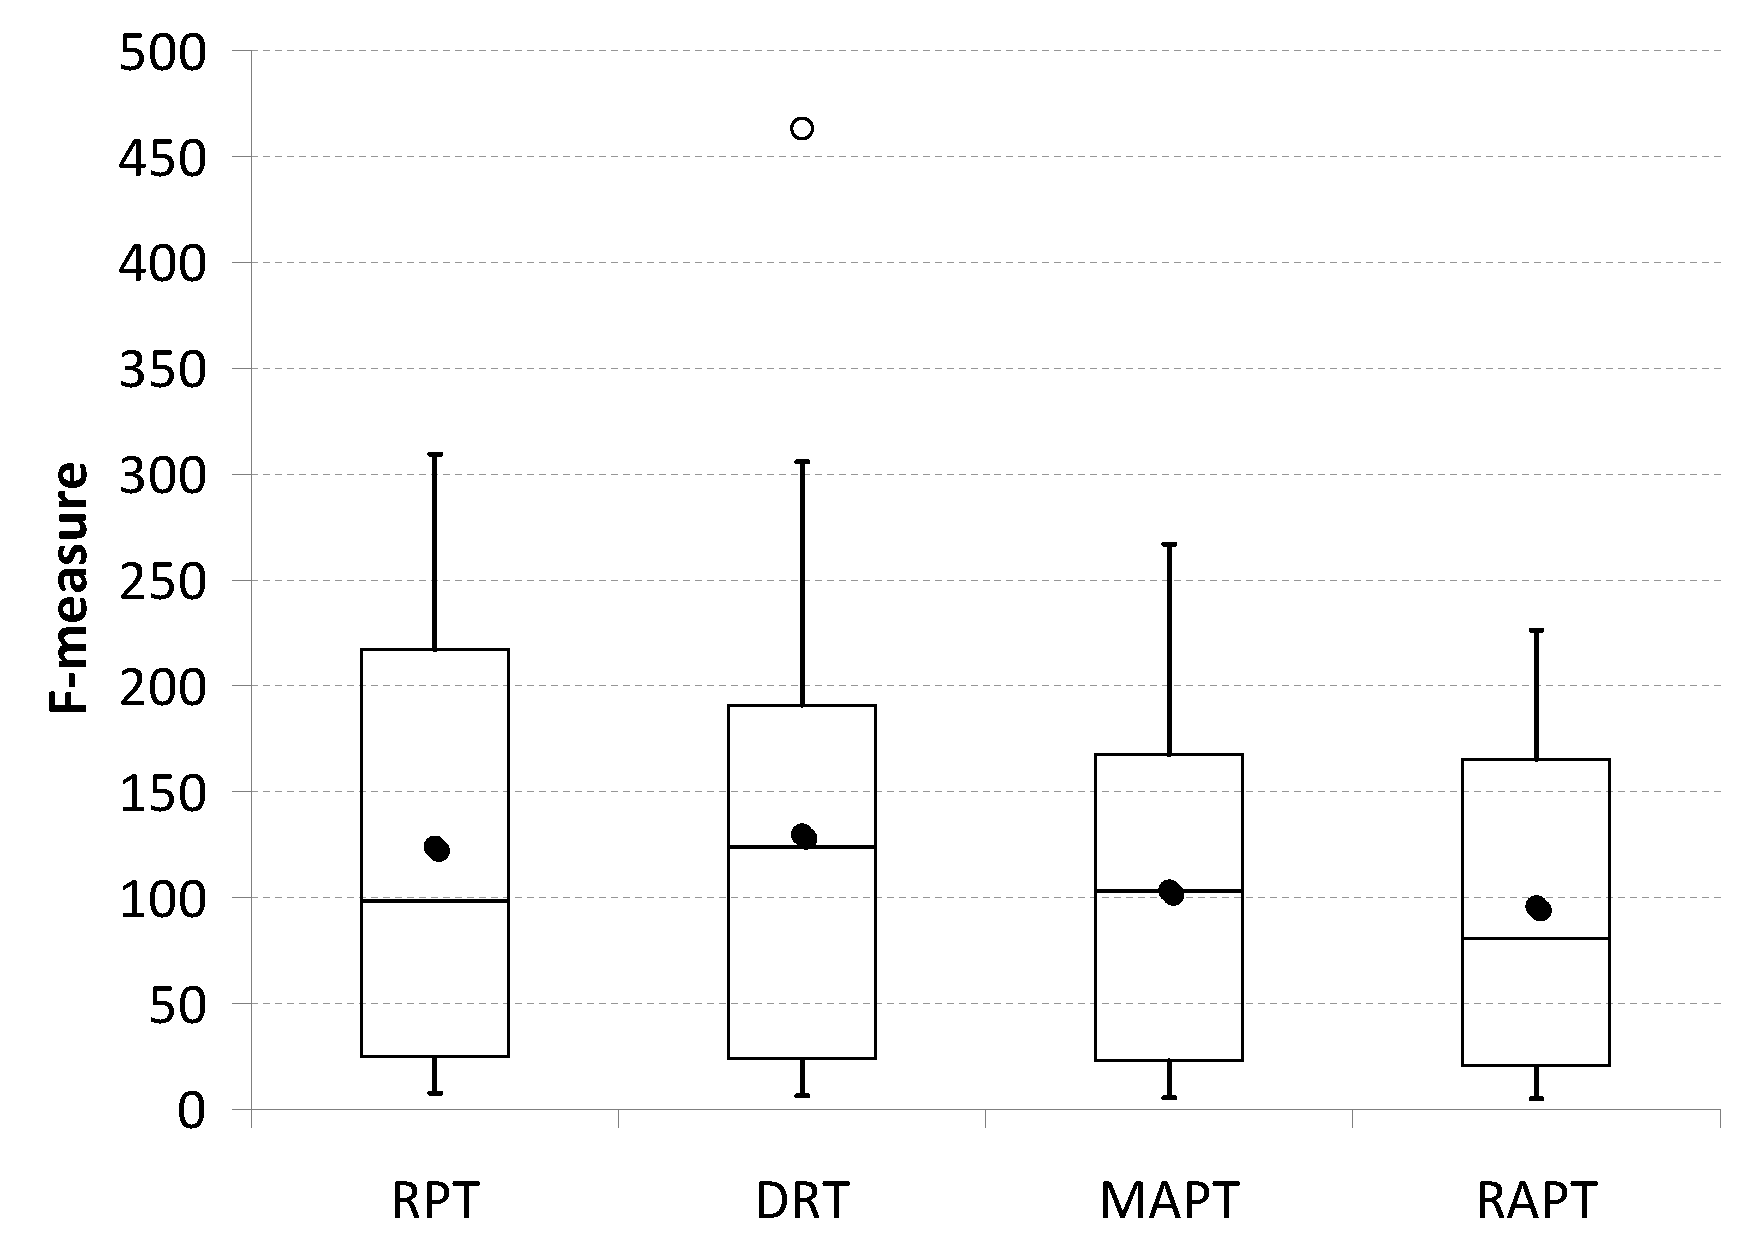
\includegraphics[width=0.32\textwidth]{grepF}}
%    \subfigure[gzip] {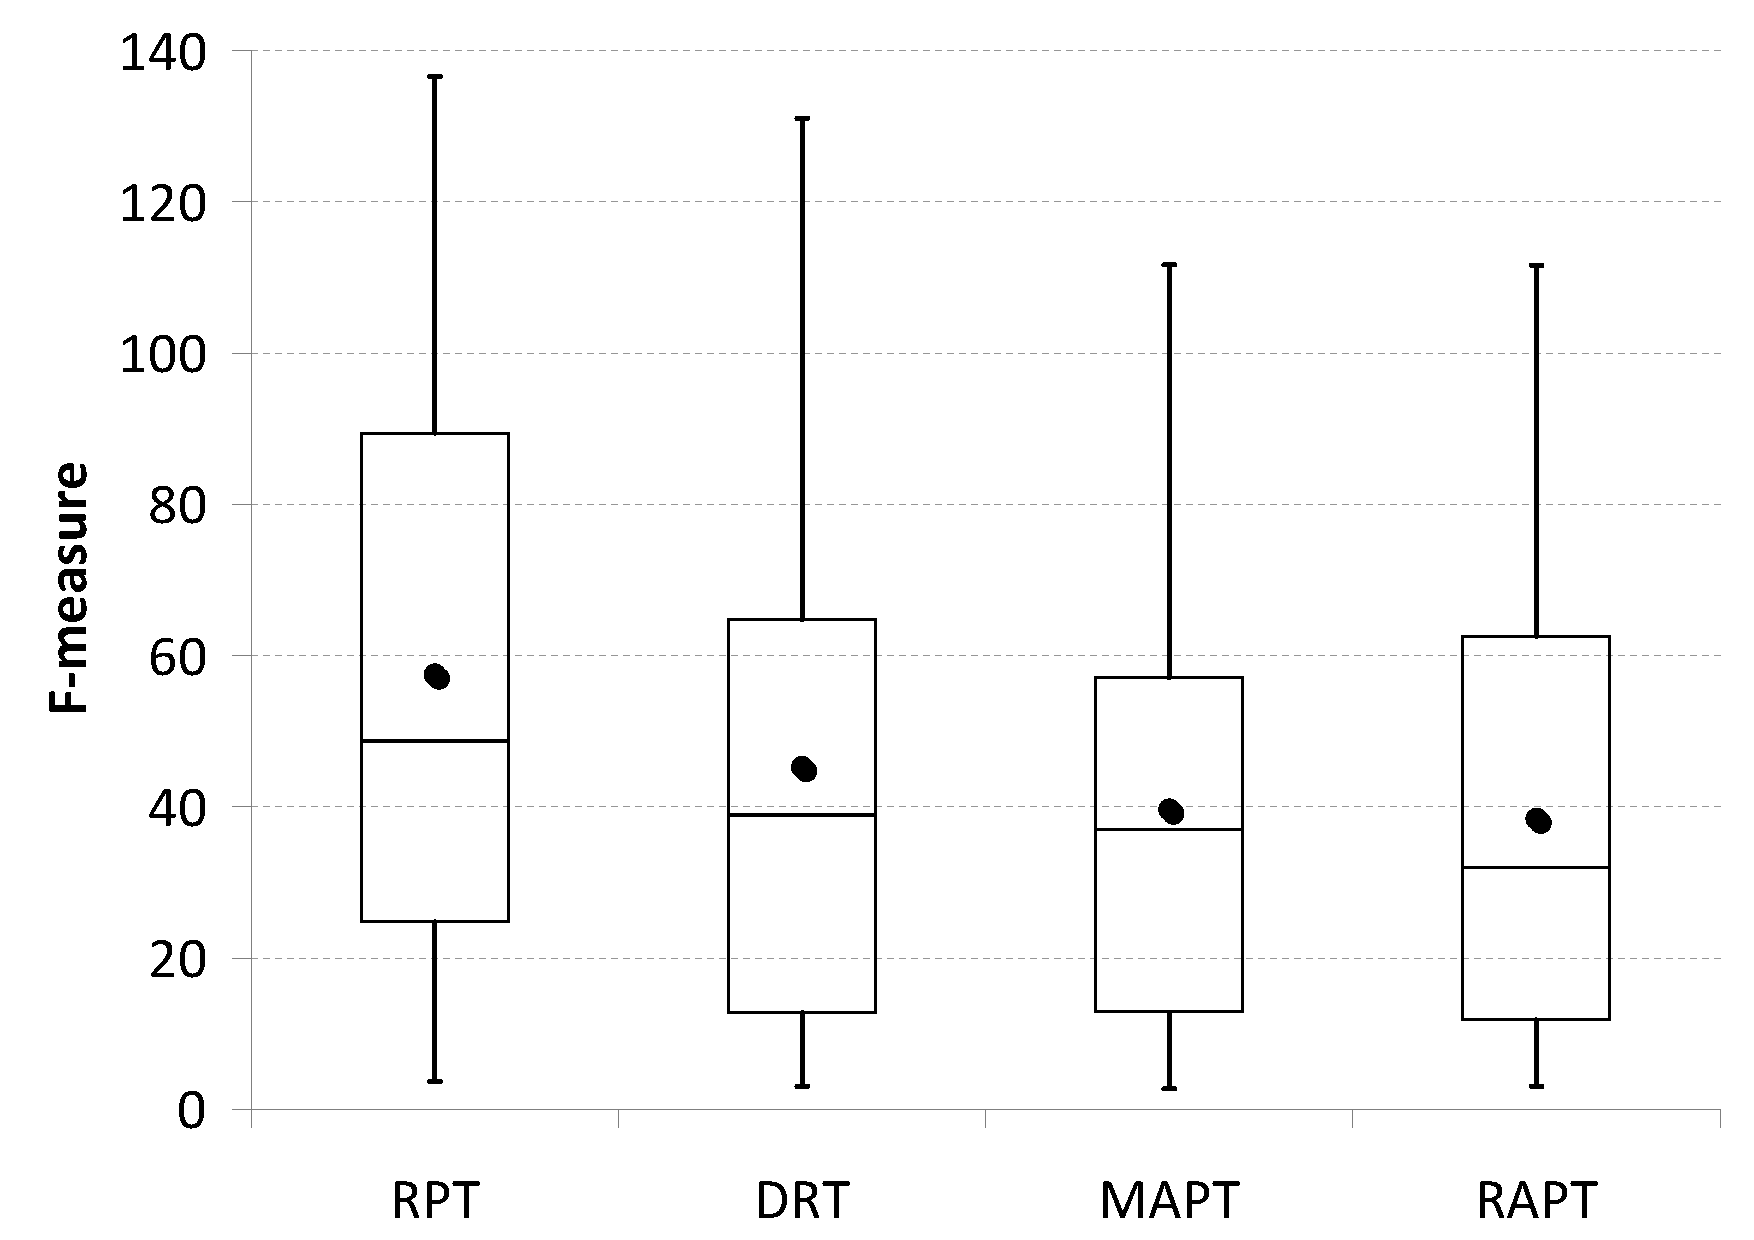
\includegraphics[width=0.32\textwidth]{gzipF}}
%    \subfigure[make] {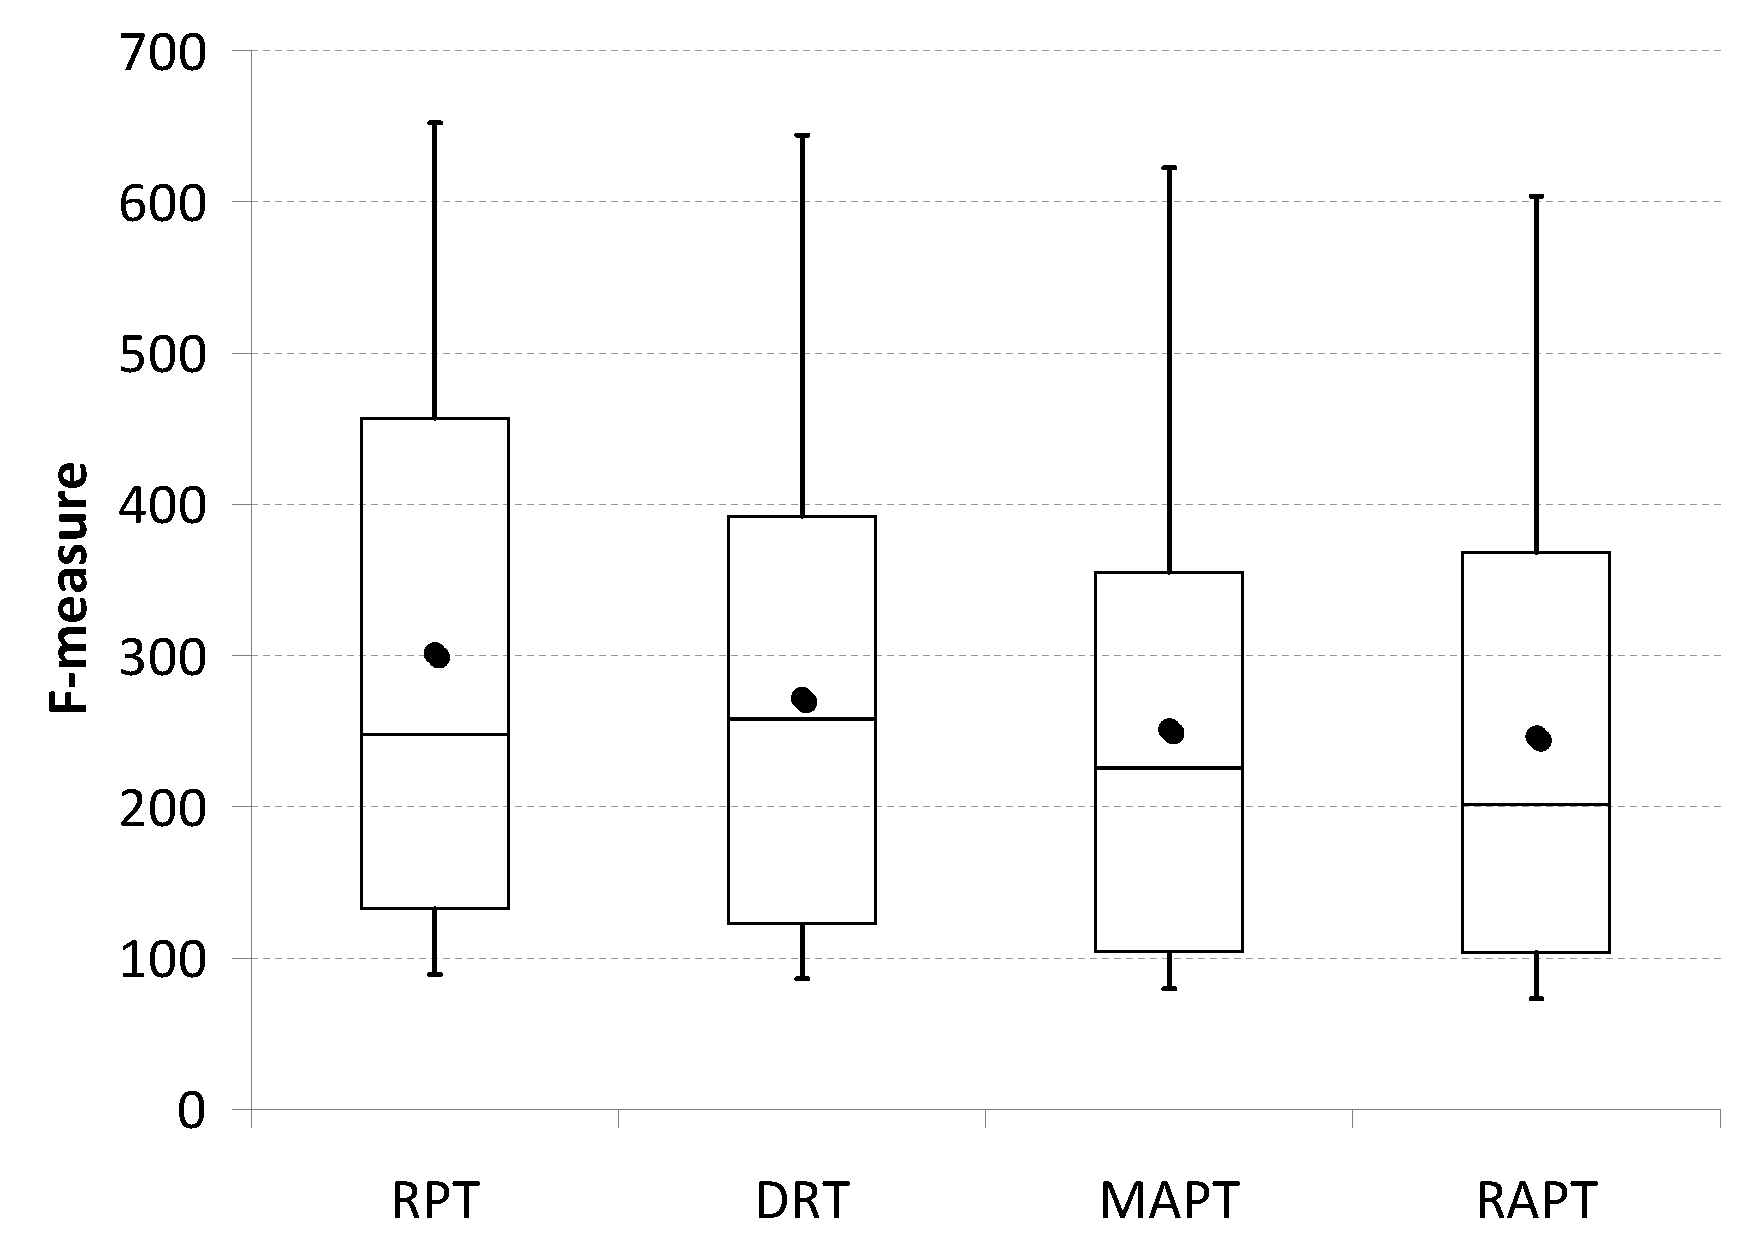
\includegraphics[width=0.32\textwidth]{makeF}}
%	\caption{Boxplots of F-measures on each object program}
%	\label{fig:Fmeasure}
%\end{figure*}
%
%\begin{figure*}[tp]
%	\centering
%	\subfigure[grep] {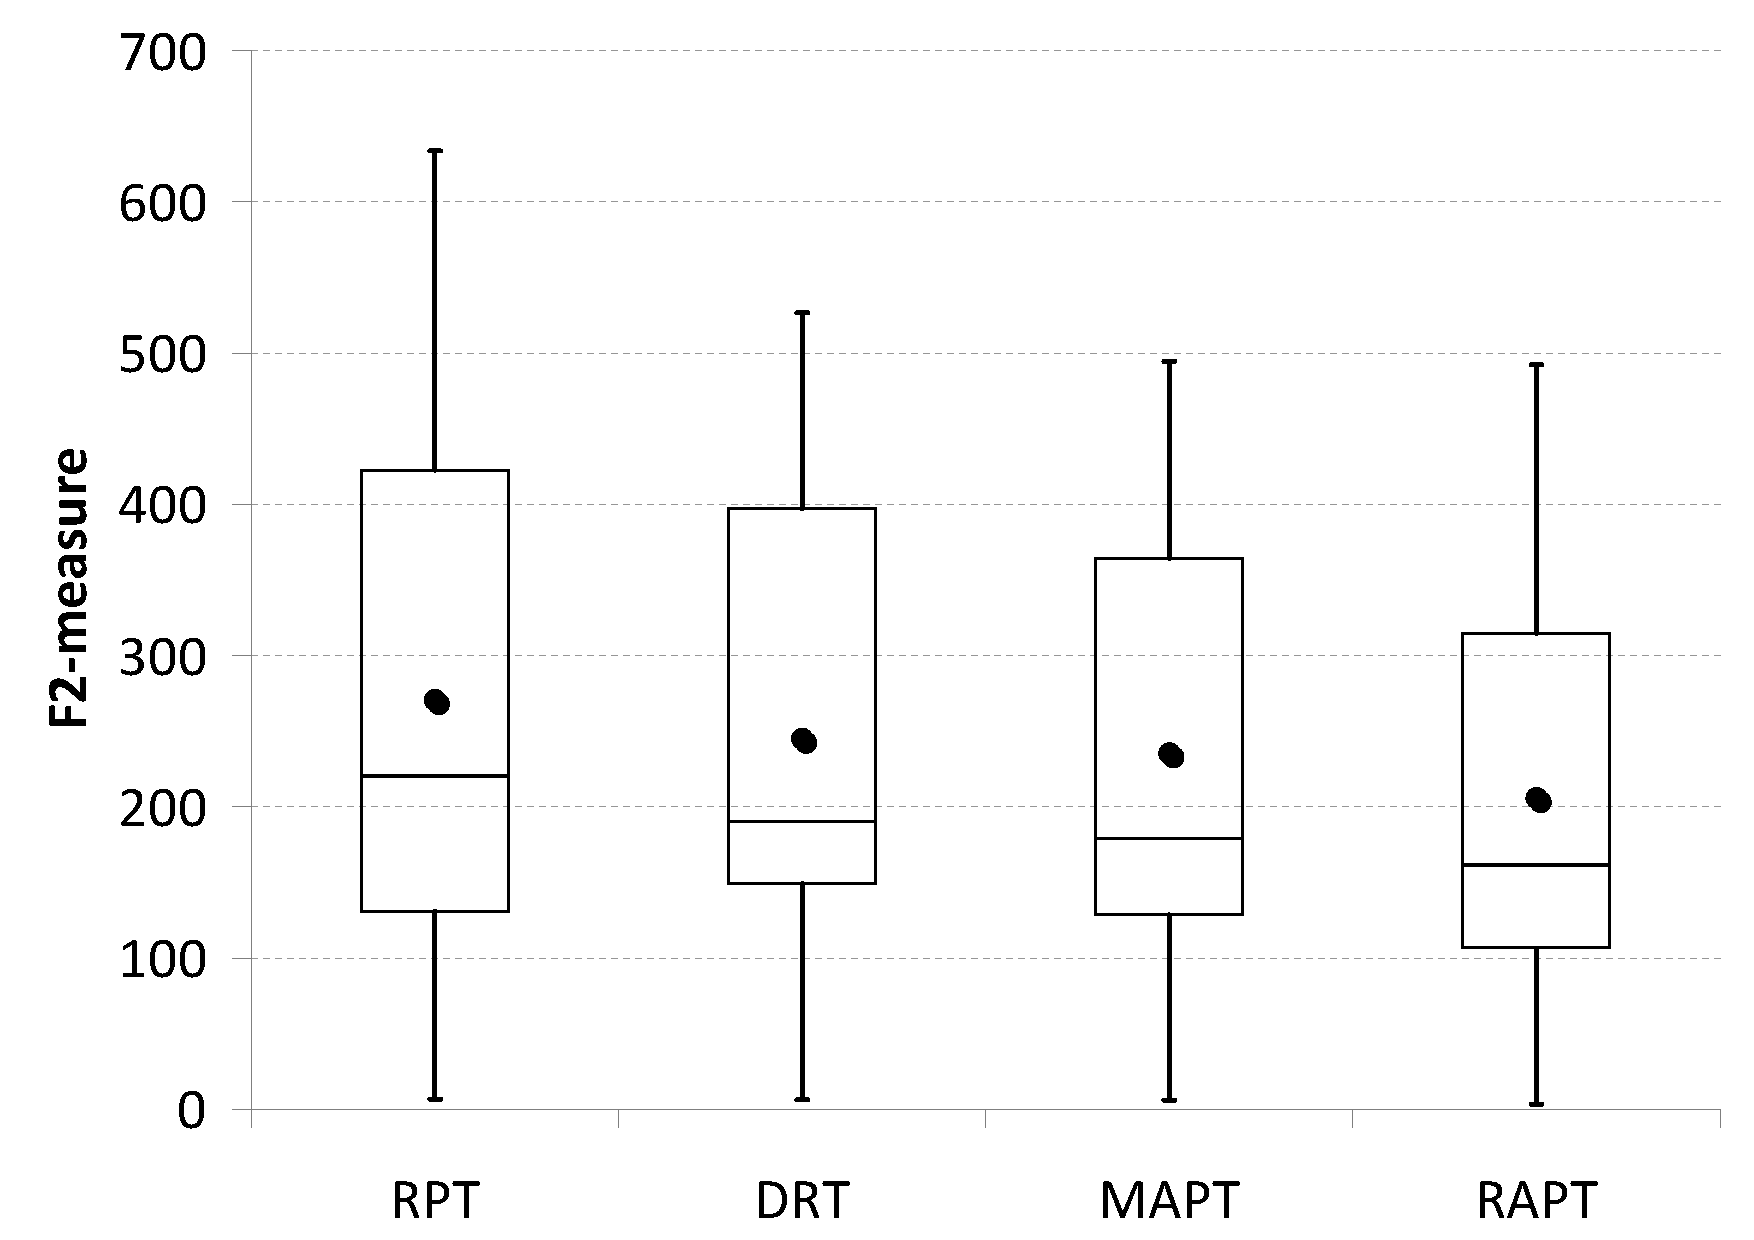
\includegraphics[width=0.32\textwidth]{grepF2}}
%    \subfigure[gzip] {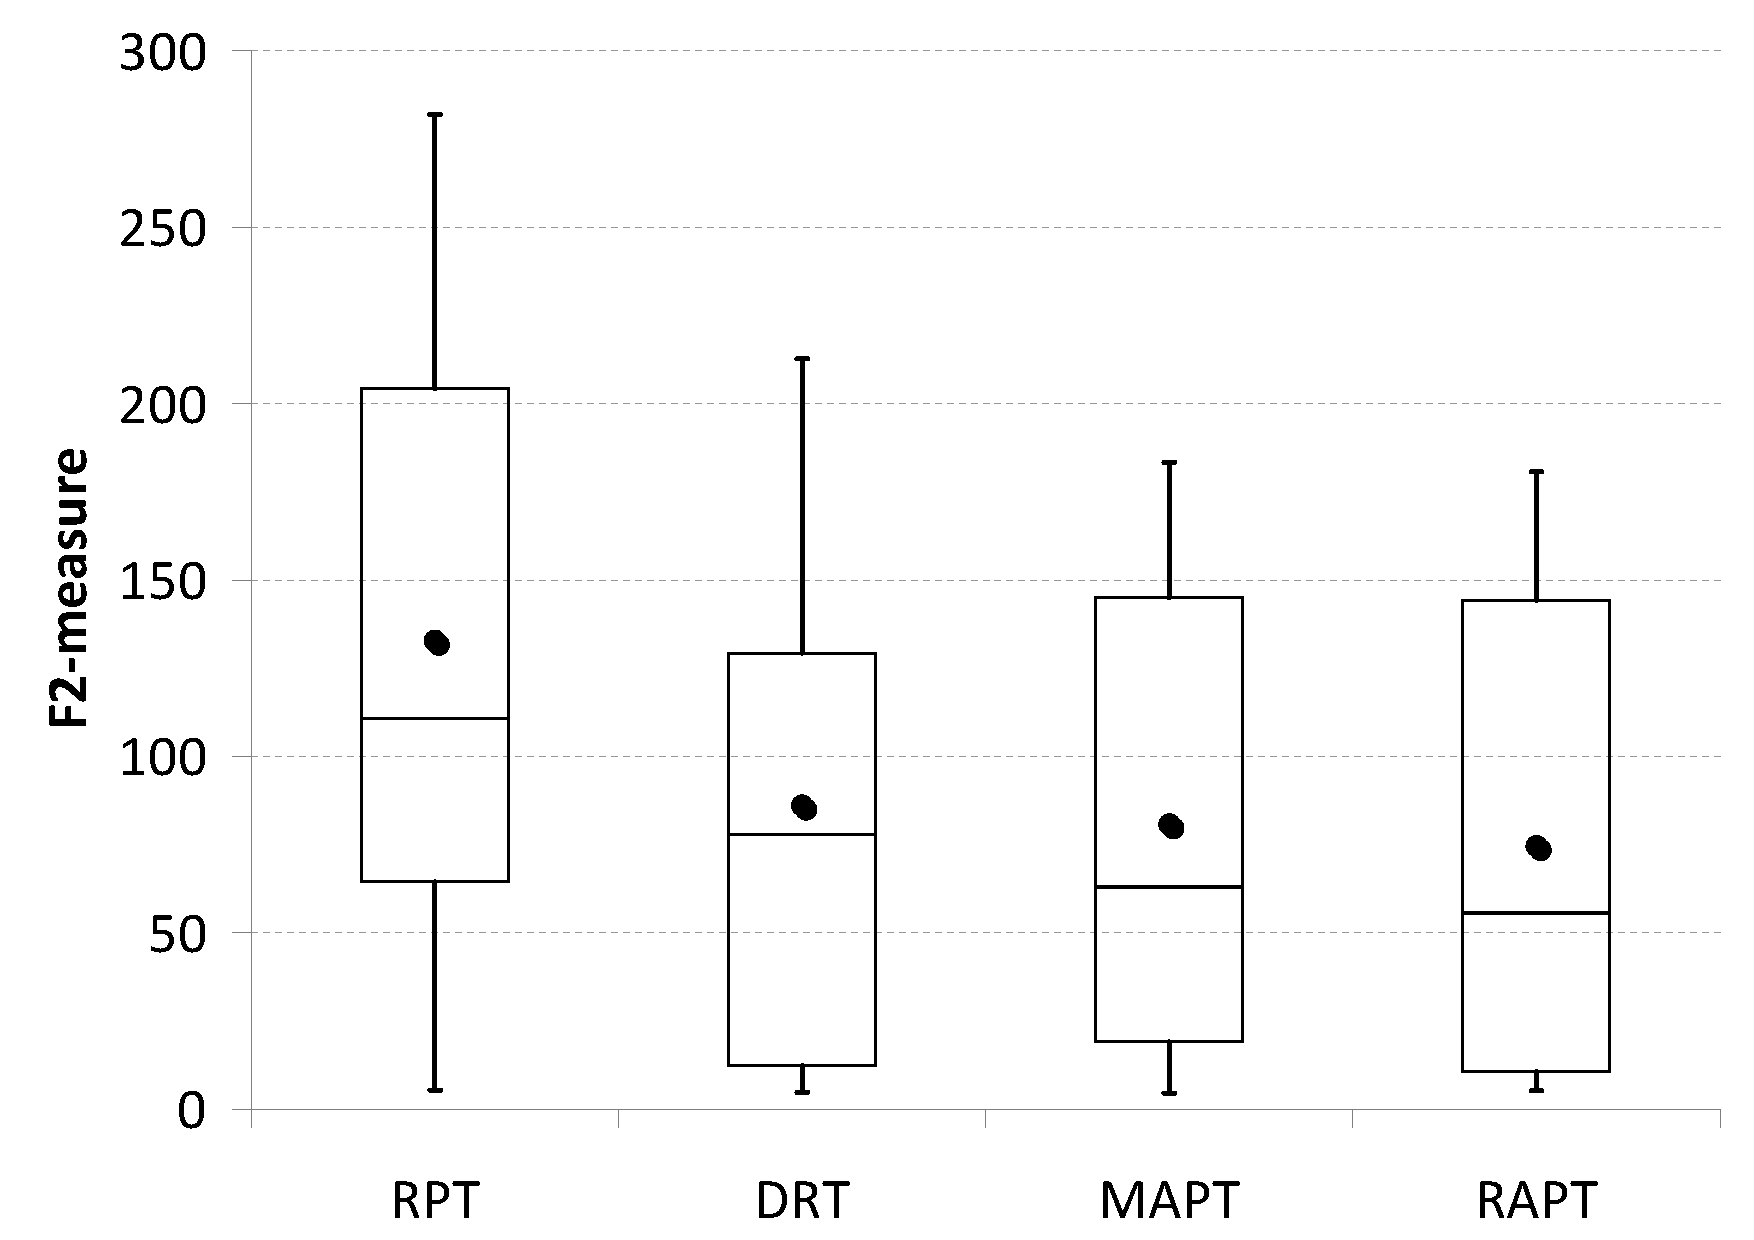
\includegraphics[width=0.32\textwidth]{gzipF2}}
%    \subfigure[make] {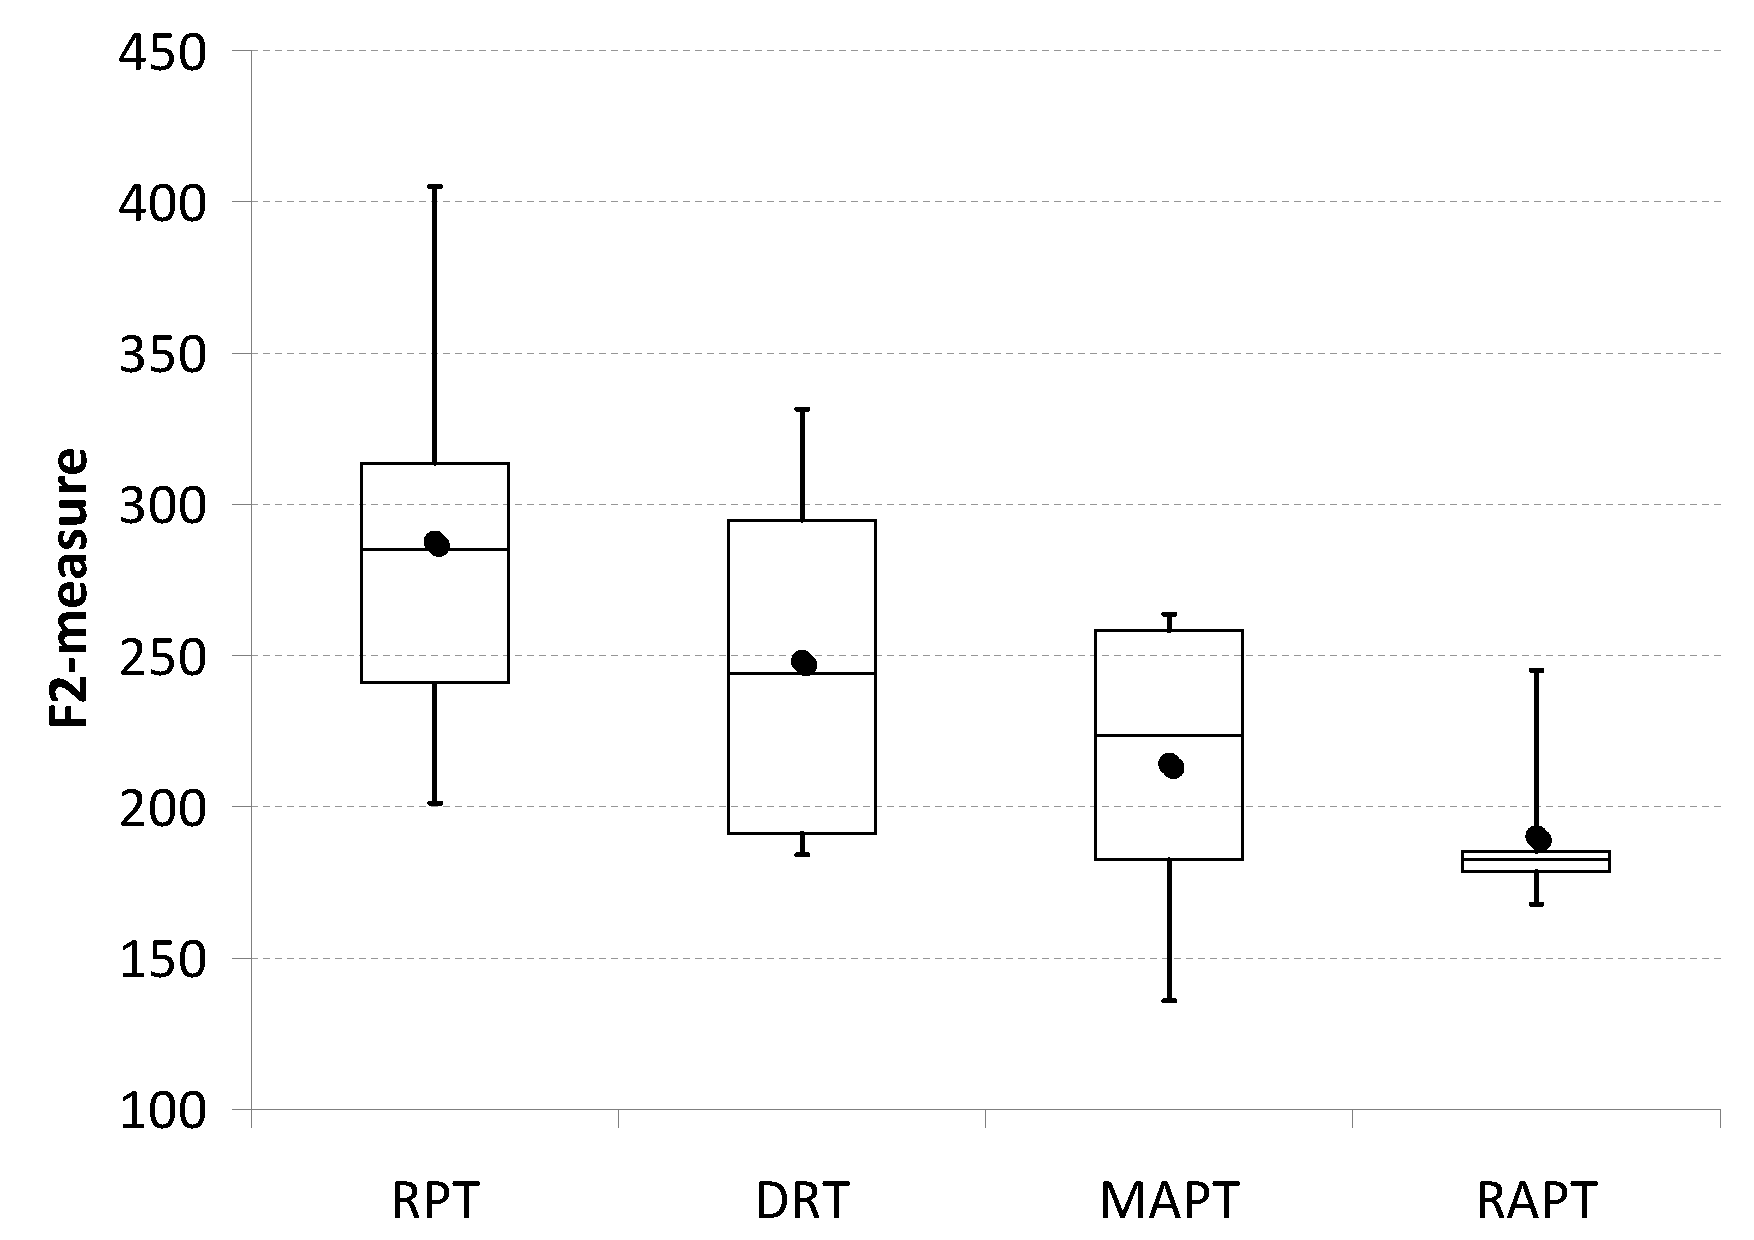
\includegraphics[width=0.32\textwidth]{makeF2}}
%	\caption{Boxplots of F2-measures on each object program}
%	\label{fig:F2measure}
%\end{figure*}
%
%From Tables~\ref{tab:Fgrep} to~\ref{tab:Fmake} and Figures~\ref{fig:Fmeasure} and~\ref{fig:F2measure}, we can observe that in general, RAPT was the best performer in terms of F-measure and F2-measure, followed by MAPT, DRT, and RPT in descending order. We further conducted statistical testing to verify the significance of this observation. We used the Holm-Bonferroni method~\cite{Holm79} (with p-value being 0.05) to determine which pair of testing techniques have significant difference. The statistical testing results are shown in Tables~\ref{tab:Fsta} and~\ref{tab:F2sta}. Each cell in the tables gives the number of scenarios where the technique on the top row performed better than that on the left column. If the difference is significant, the number will be displayed in bold. For example, the bold 59 in the top right corner in Table~\ref{tab:Fsta} indicates that out of 60 scenarios (10 faulty versions $\times$ 3 granularities $\times$ 2 initial profiles), RAPT had smaller F-measure than RPT for 59 scenarios, and the fault-detection capabilities of these two techniques were significantly different.
%
%\begin{table}
%\caption{Number of scenarios where the technique on top row has smaller F-measure than that on left column}
%\label{tab:Fsta}
%\centering
%\begin{tabular}{|c|c|c|c|c|} \hline
%			& RPT					& DRT					& MAPT				& RAPT				\\ \hline
%RPT		& ---					& \textbf{49}	& \textbf{59}	& \textbf{59}	\\ \hline
%DRT		& \textbf{11}	& ---					& \textbf{56}	& \textbf{55}	\\ \hline
%MAPT	& \textbf{1}	& \textbf{4}	& ---					& \textbf{40}	\\ \hline
%RAPT	& \textbf{1}	& \textbf{5}	& \textbf{20}	& ---					\\ \hline
%\end{tabular}
%\end{table}
%
%\begin{table}
%\caption{Number of scenarios where the technique on top row has smaller F2-measure than that on left column}
%\label{tab:F2sta}
%\centering
%\begin{tabular}{|c|c|c|c|c|} \hline
%			& RPT					& DRT					& MAPT				& RAPT				\\ \hline
%RPT		& ---					& \textbf{31}	& \textbf{36}	& \textbf{36}	\\ \hline
%DRT		& \textbf{11}	& ---					& \textbf{33}	& \textbf{38}	\\ \hline
%MAPT	& \textbf{6}	& \textbf{9}	& ---					& \textbf{33}	\\ \hline
%RAPT	& \textbf{6}	& \textbf{4}	& \textbf{9}	& ---					\\ \hline
%\end{tabular}
%\end{table}
%
%Tables~\ref{tab:Fsta} and~\ref{tab:F2sta} clearly show that the effectiveness difference between each pair of testing techniques was always significantly different.
%
%\subsection{RQ2: Selection overhead}

%The experimental results of T-measure and T2-measure are summarized in Tables~\ref{tab:Tgrep} to~\ref{tab:Tmake}.

%and their distributions on each object program are plotted in Figures~\ref{fig:Tmeasure} and~\ref{fig:T2measure}.

\begin{table*}
\caption{T-measure and T2-measure for program \texttt{grep} (in ms) (a lower score indicating better performance)}
\label{tab:Tgrep}
\centering
\begin{tabular}{|c|l|l|c|c|c|c|c|c|c|c|} \hline
Version	& Granularity	& Probability Profile	& $T_{RPT}$	& $T_{DRT}$	& $T_{MAPT}$	& $T_{RAPT}$	& $T2_{RPT}$	& $T2_{DRT}$	& $T2_{MAPT}$	 & $T2_{RAPT}$	\\ \hline
V1	& Coarse	& Equal	& 31102.30	& 42012.50	& 28664.75	& 11612.00	& 68868.95	& 92326.45	& 100426.90	& 39167.70	 \\ \cline{3-11}
	& 	& Proportional	& 21725.95	& 13495.60	& 12048.55	& 12495.15	& 57600.10	& 46176.00	& 57060.50	& 35818.40	 \\ \cline{2-11}
	& Medium	& Equal	& 84986.85	& 72931.35	& 79151.65	& 50351.80	& 46526.90	& 51245.85	& 18892.60	& 56496.00	 \\ \cline{3-11}
	& 	& Proportional	& 15752.40	& 16537.25	& 12356.45	& 14378.30	& 41629.05	& 53319.90	& 27628.75	& 31196.90	 \\ \cline{2-11}
	& Fine	& Equal	& 58478.50	& 31922.00	& 48094.75	& 18791.20	& 33589.15	& 44661.20	& 40473.25	& 52750.15	 \\ \cline{3-11}
	& 	& Proportional	& 12503.05	& 17547.10	& 7835.05	& 18823.45	& 18188.60	& 36484.50	& 16433.15	& 43683.15	 \\ \hline
V2	& Coarse	& Equal	& 3022.20	& 4415.65	& 3168.55	& 1844.20	& 29962.50	& 34308.80	& 37136.85	& 18567.00	 \\ \cline{3-11}
	& 	& Proportional	& 811.65	& 1223.70	& 537.80	& 1078.00	& 12982.15	& 45877.20	& 20286.75	& 19894.30	 \\ \cline{2-11}
	& Medium	& Equal	& 2843.60	& 3828.75	& 3095.25	& 2332.25	& 2534.15	& 5803.50	& 5220.65	& 2518.00	 \\ \cline{3-11}
	& 	& Proportional	& 1182.95	& 1903.95	& 1860.25	& 1432.55	& 17720.95	& 28450.80	& 18347.85	& 20247.50	 \\ \cline{2-11}
	& Fine	& Equal	& 2579.05	& 6441.80	& 3117.60	& 2658.90	& 1831.10	& 11332.50	& 9511.40	& 1854.05	 \\ \cline{3-11}
	& 	& Proportional	& 2743.55	& 2866.55	& 2610.40	& 2755.20	& 31521.90	& 31005.70	& 35737.65	& 26285.10	 \\ \hline
V3	& Coarse	& Equal	& 13422.30	& 10835.85	& 7896.20	& 5919.00	& 51203.60	& 69810.05	& 50489.90	& 13097.75	 \\ \cline{3-11}
	& 	& Proportional	& 3717.25	& 6593.70	& 3150.85	& 5161.30	& 13191.05	& 21866.05	& 11114.40	& 15047.45	 \\ \cline{2-11}
	& Medium	& Equal	& 69899.25	& 96427.20	& 79616.80	& 32076.20	& 56034.20	& 139706.50	& 120935.00	& 43150.30	 \\ \cline{3-11}
	& 	& Proportional	& 5874.45	& 4318.60	& 6227.90	& 5592.10	& 26637.75	& 23314.20	& 25535.75	& 11720.25	 \\ \cline{2-11}
	& Fine	& Equal	& 37761.20	& 31888.50	& 27193.40	& 18876.40	& 56283.05	& 65960.15	& 54118.80	& 35059.80	 \\ \cline{3-11}
	& 	& Proportional	& 6702.20	& 5746.50	& 3958.15	& 6078.80	& 21295.25	& 16642.10	& 16559.65	& 13966.10	 \\ \hline
V4	& Coarse	& Equal	& 107716.40	& 147239.30	& 79275.05	& 43325.40	& ---	& ---	& ---	& ---	 \\ \cline{3-11}
	& 	& Proportional	& 21786.25	& 27050.20	& 25651.10	& 21454.40	& ---	& ---	& ---	& ---	 \\ \cline{2-11}
	& Medium	& Equal	& 164911.80	& 79536.40	& 125860.80	& 82878.65	& ---	& ---	& ---	& ---	 \\ \cline{3-11}
	& 	& Proportional	& 24497.05	& 38017.75	& 26851.50	& 39399.80	& ---	& ---	& ---	& ---	 \\ \cline{2-11}
	& Fine	& Equal	& 74948.05	& 73944.20	& 65696.75	& 63661.50	& ---	& ---	& ---	& ---	 \\ \cline{3-11}
	& 	& Proportional	& 18328.60	& 29748.75	& 10106.05	& 23645.80	& ---	& ---	& ---	& ---	 \\ \hline
\end{tabular}
\end{table*}

\begin{table*}
\caption{T-measure and T2-measure for program \texttt{gzip} (in ms)(a lower score indicating better performance)}
\label{tab:Tgzip}
\centering
\begin{tabular}{|c|l|l|c|c|c|c|c|c|c|c|} \hline
Version	& Granularity	& Probability Profile	& $T_{RPT}$	& $T_{DRT}$	& $T_{MAPT}$	& $T_{RAPT}$	& $T2_{RPT}$	& $T2_{DRT}$	& $T2_{MAPT}$	 & $T2_{RAPT}$	\\ \hline
V1	& Coarse	& Equal	& 14506.65	& 13006.65	& 10075.45	& 6705.15	& 29848.35	& 29461.30	& 28869.75	& 9591.55	 \\ \cline{3-11}
	& 	& Proportional	& 17718.85	& 18644.75	& 12794.95	& 18777.05	& 69503.50	& 51049.15	& 26623.15	& 26533.60	 \\ \cline{2-11}
	& Medium	& Equal	& 28379.20	& 13594.40	& 16802.70	& 14489.40	& 33630.05	& 29076.75	& 29168.65	& 10984.10	 \\ \cline{3-11}
	& 	& Proportional	& 14626.20	& 6896.25	& 12403.95	& 11807.35	& 32338.85	& 14297.10	& 26989.25	& 11013.00	 \\ \cline{2-11}
	& Fine	& Equal	& 26610.95	& 28794.00	& 31465.30	& 13850.20	& 80868.80	& 72540.55	& 72624.35	& 80242.65	 \\ \cline{3-11}
	& 	& Proportional	& 18458.00	& 20173.95	& 22114.00	& 6936.00	& 32638.30	& 19971.25	& 29493.10	& 25842.15	 \\ \hline
V2	& Coarse	& Equal	& 44281.65	& 28899.00	& 21174.20	& 13910.10	& ---	& ---	& ---	& ---	 \\ \cline{3-11}
	& 	& Proportional	& 4148.55	& 5759.25	& 5397.55	& 5453.05	& ---	& ---	& ---	& ---	 \\ \cline{2-11}
	& Medium	& Equal	& 34312.00	& 17583.25	& 21040.25	& 30294.05	& ---	& ---	& ---	& ---	 \\ \cline{3-11}
	& 	& Proportional	& 5175.95	& 2702.50	& 4563.70	& 4077.10	& ---	& ---	& ---	& ---	 \\ \cline{2-11}
	& Fine	& Equal	& 20329.20	& 26648.35	& 20355.75	& 10805.35	& ---	& ---	& ---	& ---	 \\ \cline{3-11}
	& 	& Proportional	& 4316.75	& 3745.45	& 3899.10	& 5203.20	& ---	& ---	& ---	& ---	 \\ \hline
V4	& Coarse	& Equal	& 29697.20	& 14206.95	& 17106.95	& 10655.00	& 47518.55	& 37240.90	& 37079.75	& 18222.20	 \\ \cline{3-11}
	& 	& Proportional	& 24748.20	& 22272.05	& 12406.85	& 19784.40	& 46939.95	& 30963.80	& 27214.65	& 21938.10	 \\ \cline{2-11}
	& Medium	& Equal	& 17356.45	& 13443.05	& 20897.45	& 12972.80	& 38900.35	& 25021.30	& 32292.40	& 26698.15	 \\ \cline{3-11}
	& 	& Proportional	& 20209.75	& 6741.30	& 15233.85	& 13068.25	& 49056.25	& 16980.25	& 24725.70	& 26000.35	 \\ \cline{2-11}
	& Fine	& Equal	& 29500.35	& 28436.65	& 34287.55	& 23942.25	& 55407.30	& 46075.05	& 43216.15	& 42009.95	 \\ \cline{3-11}
	& 	& Proportional	& 20751.30	& 33156.75	& 16290.15	& 15935.75	& 27408.35	& 37622.90	& 45239.95	& 43791.80	 \\ \hline
V5	& Coarse	& Equal	& 2792.45	& 2730.10	& 2909.85	& 2383.65	& 6258.95	& 4514.10	& 6117.60	& 5369.75	 \\ \cline{3-11}
	& 	& Proportional	& 15881.40	& 5670.25	& 9080.00	& 6337.80	& 19868.30	& 7631.85	& 8996.60	& 6390.30	 \\ \cline{2-11}
	& Medium	& Equal	& 1927.10	& 1551.80	& 1979.30	& 1930.60	& 5354.55	& 2667.80	& 5040.60	& 4827.40	 \\ \cline{3-11}
	& 	& Proportional	& 11345.90	& 2078.40	& 3550.85	& 3956.90	& 18939.40	& 2768.55	& 15227.40	& 7302.95	 \\ \cline{2-11}
	& Fine	& Equal	& 3091.95	& 4660.15	& 3834.85	& 3487.35	& 8543.50	& 8470.80	& 7861.85	& 8109.00	 \\ \cline{3-11}
	& 	& Proportional	& 13897.55	& 5918.45	& 7772.65	& 5844.20	& 19799.75	& 6421.65	& 9634.80	& 9634.80	 \\ \hline
\end{tabular}
\end{table*}

\begin{table*}
\caption{T-measure and T2-measure for program \texttt{make} (in ms)(a lower score indicating better performance)}
\label{tab:Tmake}
\centering
\begin{tabular}{|c|l|l|c|c|c|c|c|c|c|c|} \hline
Version	& Granularity	& Probability Profile	& $T_{RPT}$	& $T_{DRT}$	& $T_{MAPT}$	& $T_{RAPT}$	& $T2_{RPT}$	& $T2_{DRT}$	& $T2_{MAPT}$	 & $T2_{RAPT}$	\\ \hline
V1	& Coarse	& Equal	& 7783.50	& 11133.95	& 7421.95	& 8142.65	& 25741.05	& 16259.55	& 18776.00	& 17920.95	 \\ \cline{3-11}
	& 	& Proportional	& 5838.55	& 10088.65	& 6558.65	& 8812.40	& 21083.90	& 16160.75	& 15463.25	& 13392.50	 \\ \cline{2-11}
	& Medium	& Equal	& 13541.70	& 10733.60	& 18753.45	& 12470.45	& 38183.05	& 30281.65	& 30210.70	& 19255.75	 \\ \cline{3-11}
	& 	& Proportional	& 10472.60	& 8560.55	& 12075.45	& 13758.75	& 19070.80	& 21337.85	& 21551.25	& 19461.15	 \\ \cline{2-11}
	& Fine	& Equal	& 21619.15	& 23385.25	& 21263.75	& 21593.25	& 27818.90	& 39644.20	& 49377.80	& 20077.70	 \\ \cline{3-11}
	& 	& Proportional	& 10112.55	& 16499.45	& 7236.95	& 8539.10	& 27387.55	& 31749.80	& 19066.05	& 11067.75	 \\ \hline
V2	& Coarse	& Equal	& 28532.75	& 35993.00	& 39727.20	& 36592.30	& ---	& ---	& ---	& ---	 \\ \cline{3-11}
	& 	& Proportional	& 20202.35	& 26408.65	& 17414.00	& 16762.60	& ---	& ---	& ---	& ---	 \\ \cline{2-11}
	& Medium	& Equal	& 20281.35	& 67205.40	& 52588.65	& 51398.40	& ---	& ---	& ---	& ---	 \\ \cline{3-11}
	& 	& Proportional	& 25628.60	& 44287.65	& 32129.30	& 25466.75	& ---	& ---	& ---	& ---	 \\ \cline{2-11}
	& Fine	& Equal	& 98311.45	& 71488.25	& 66706.65	& 45466.25	& ---	& ---	& ---	& ---	 \\ \cline{3-11}
	& 	& Proportional	& 48635.00	& 25699.85	& 54519.25	& 60452.05	& ---	& ---	& ---	& ---	 \\ \hline
\end{tabular}
\end{table*}

%\begin{figure*}[tp]
%	\centering
%	\subfigure[grep] {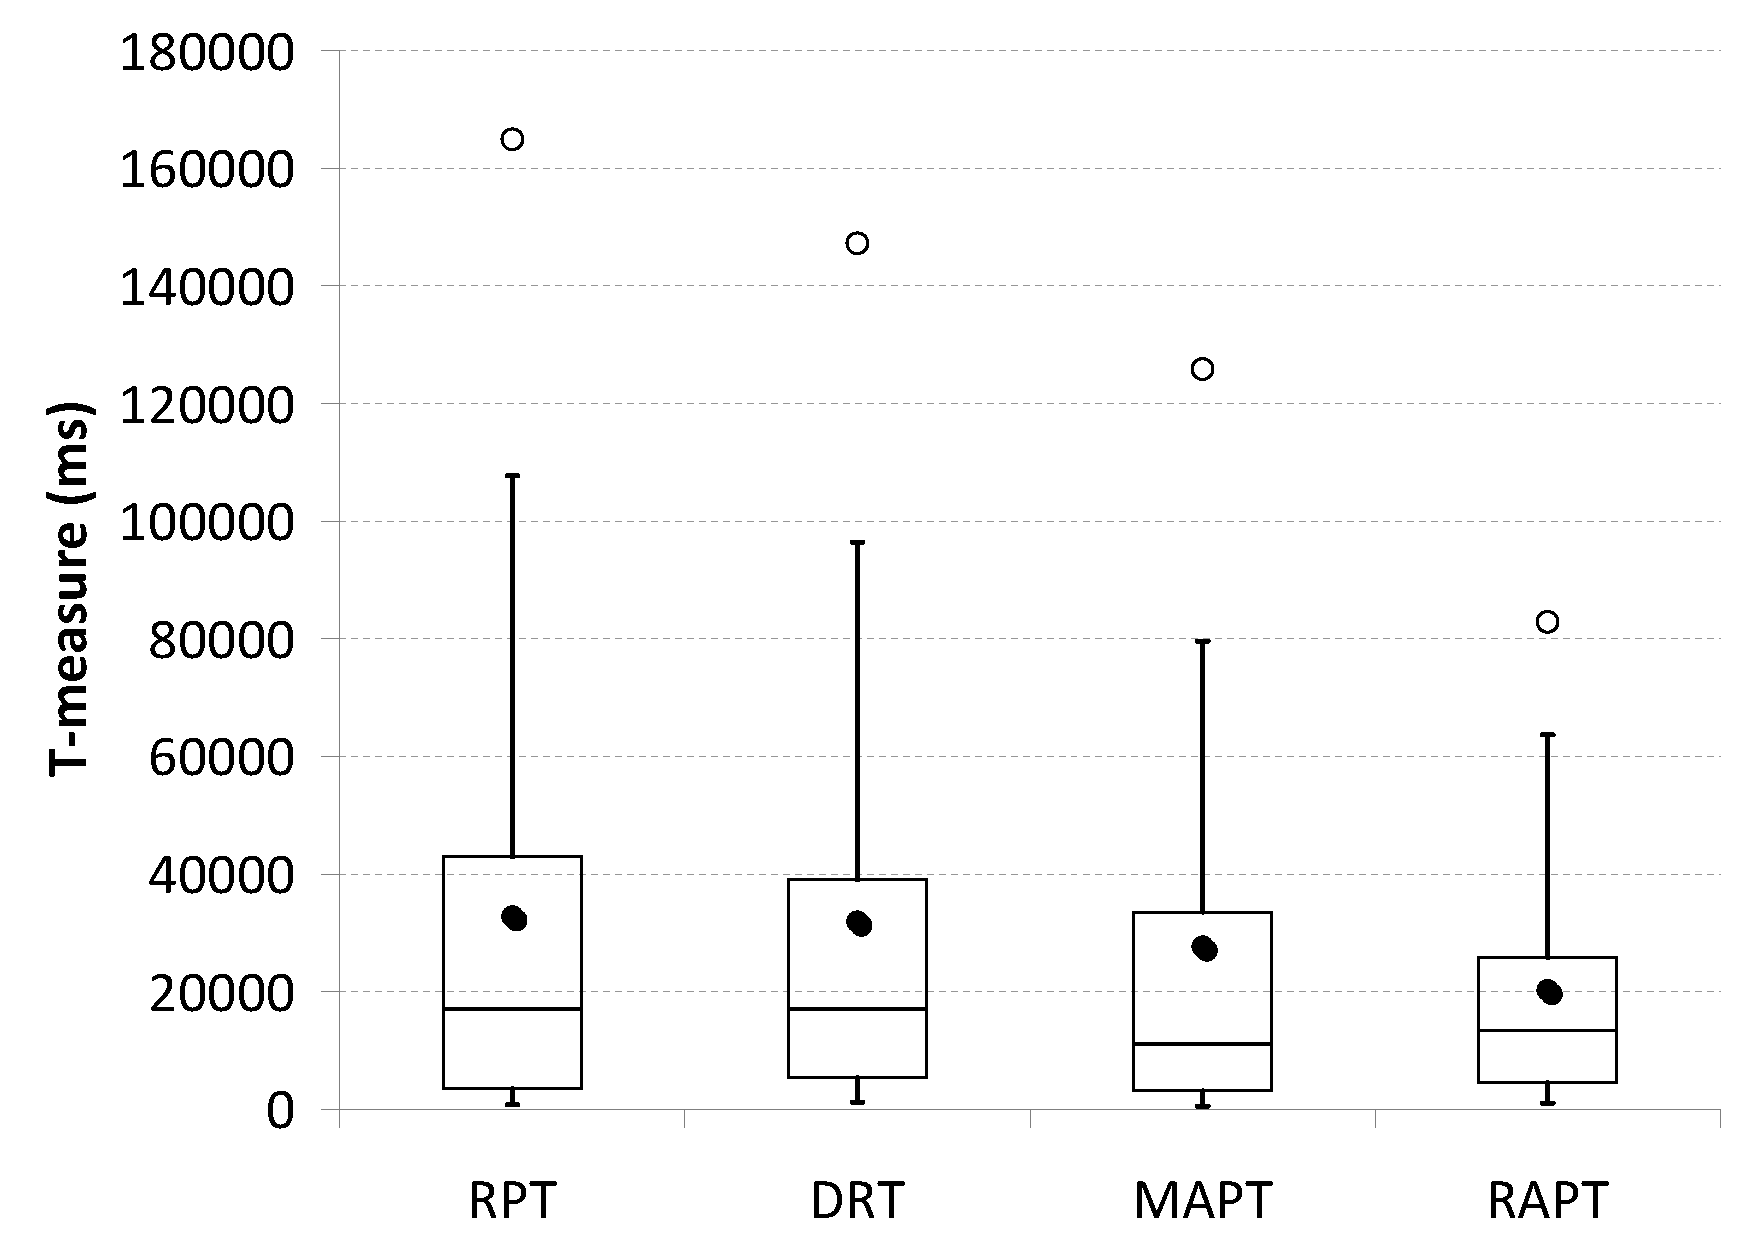
\includegraphics[width=0.32\textwidth]{grepT}}
%    \subfigure[gzip] {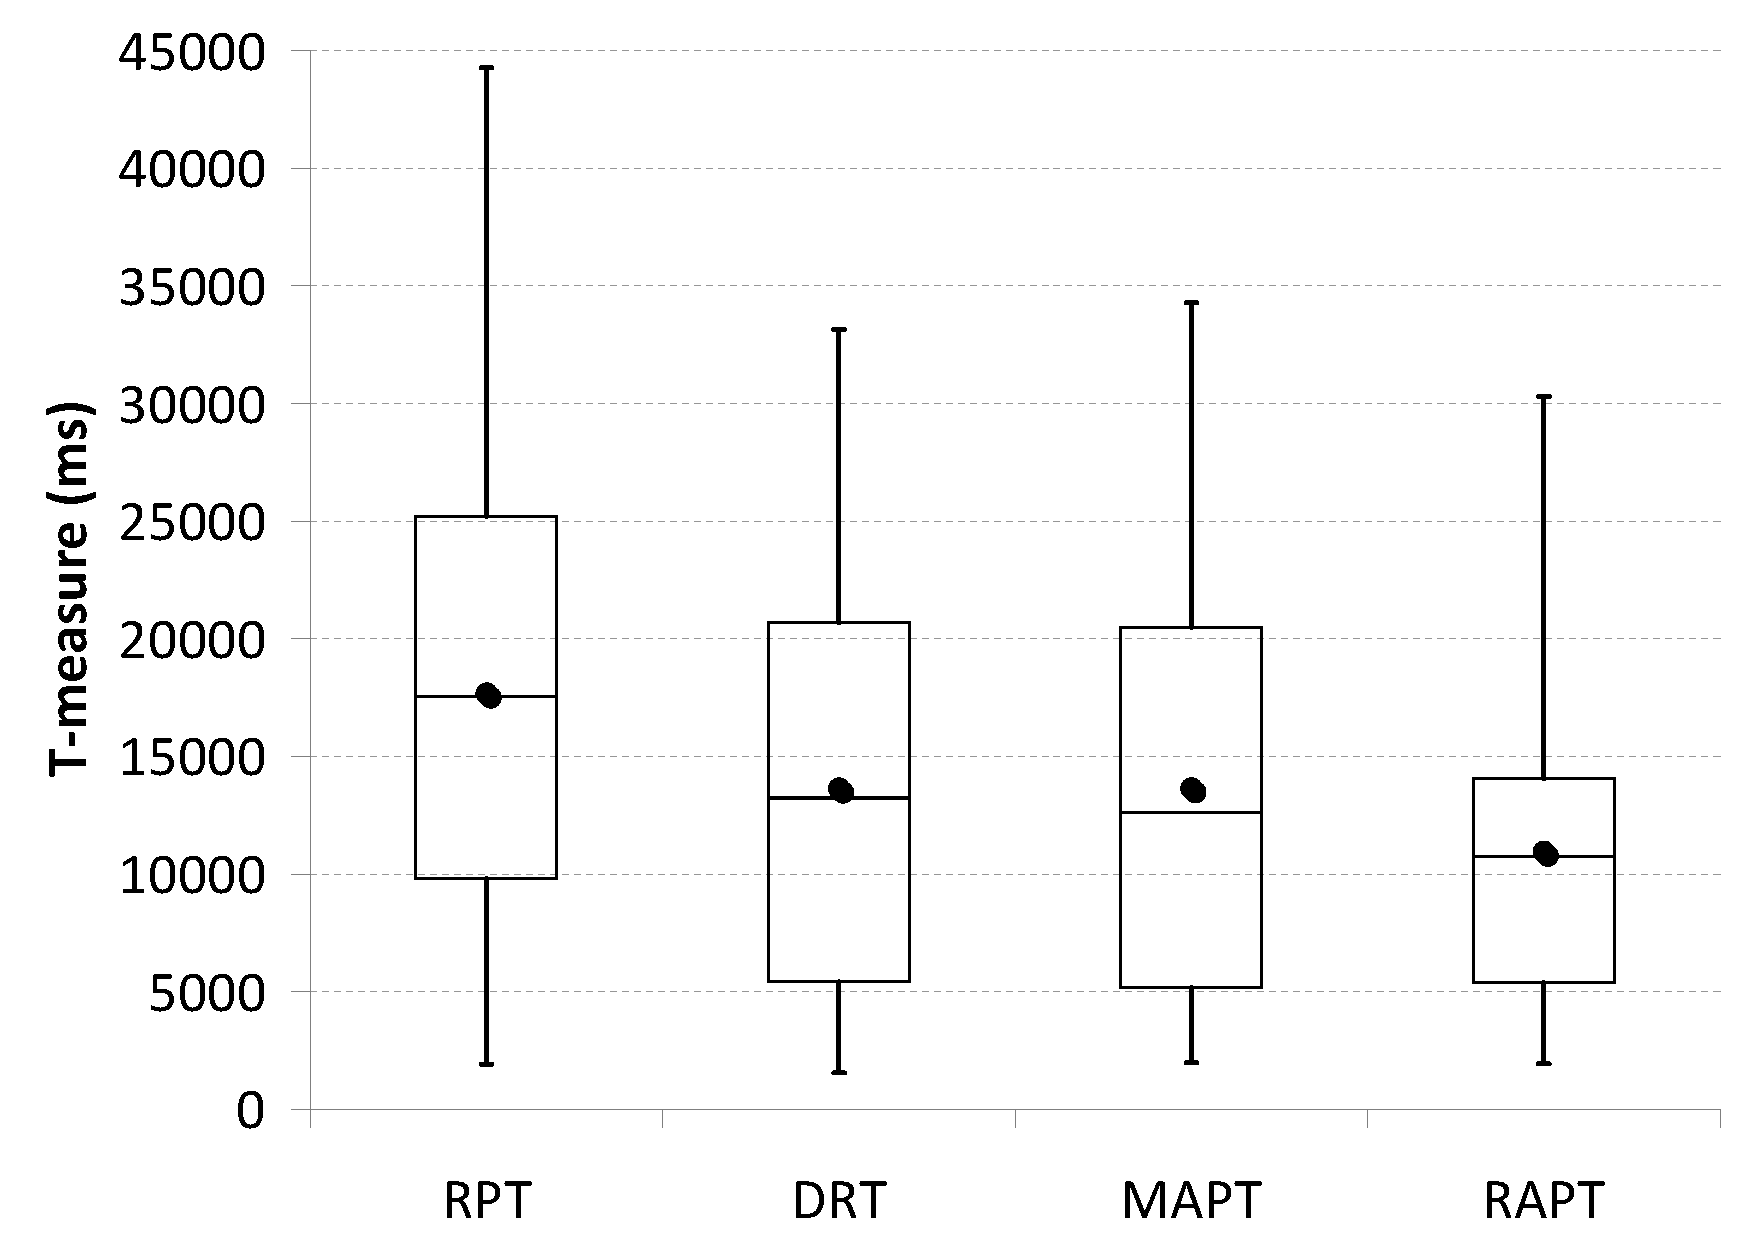
\includegraphics[width=0.32\textwidth]{gzipT}}
%    \subfigure[make] {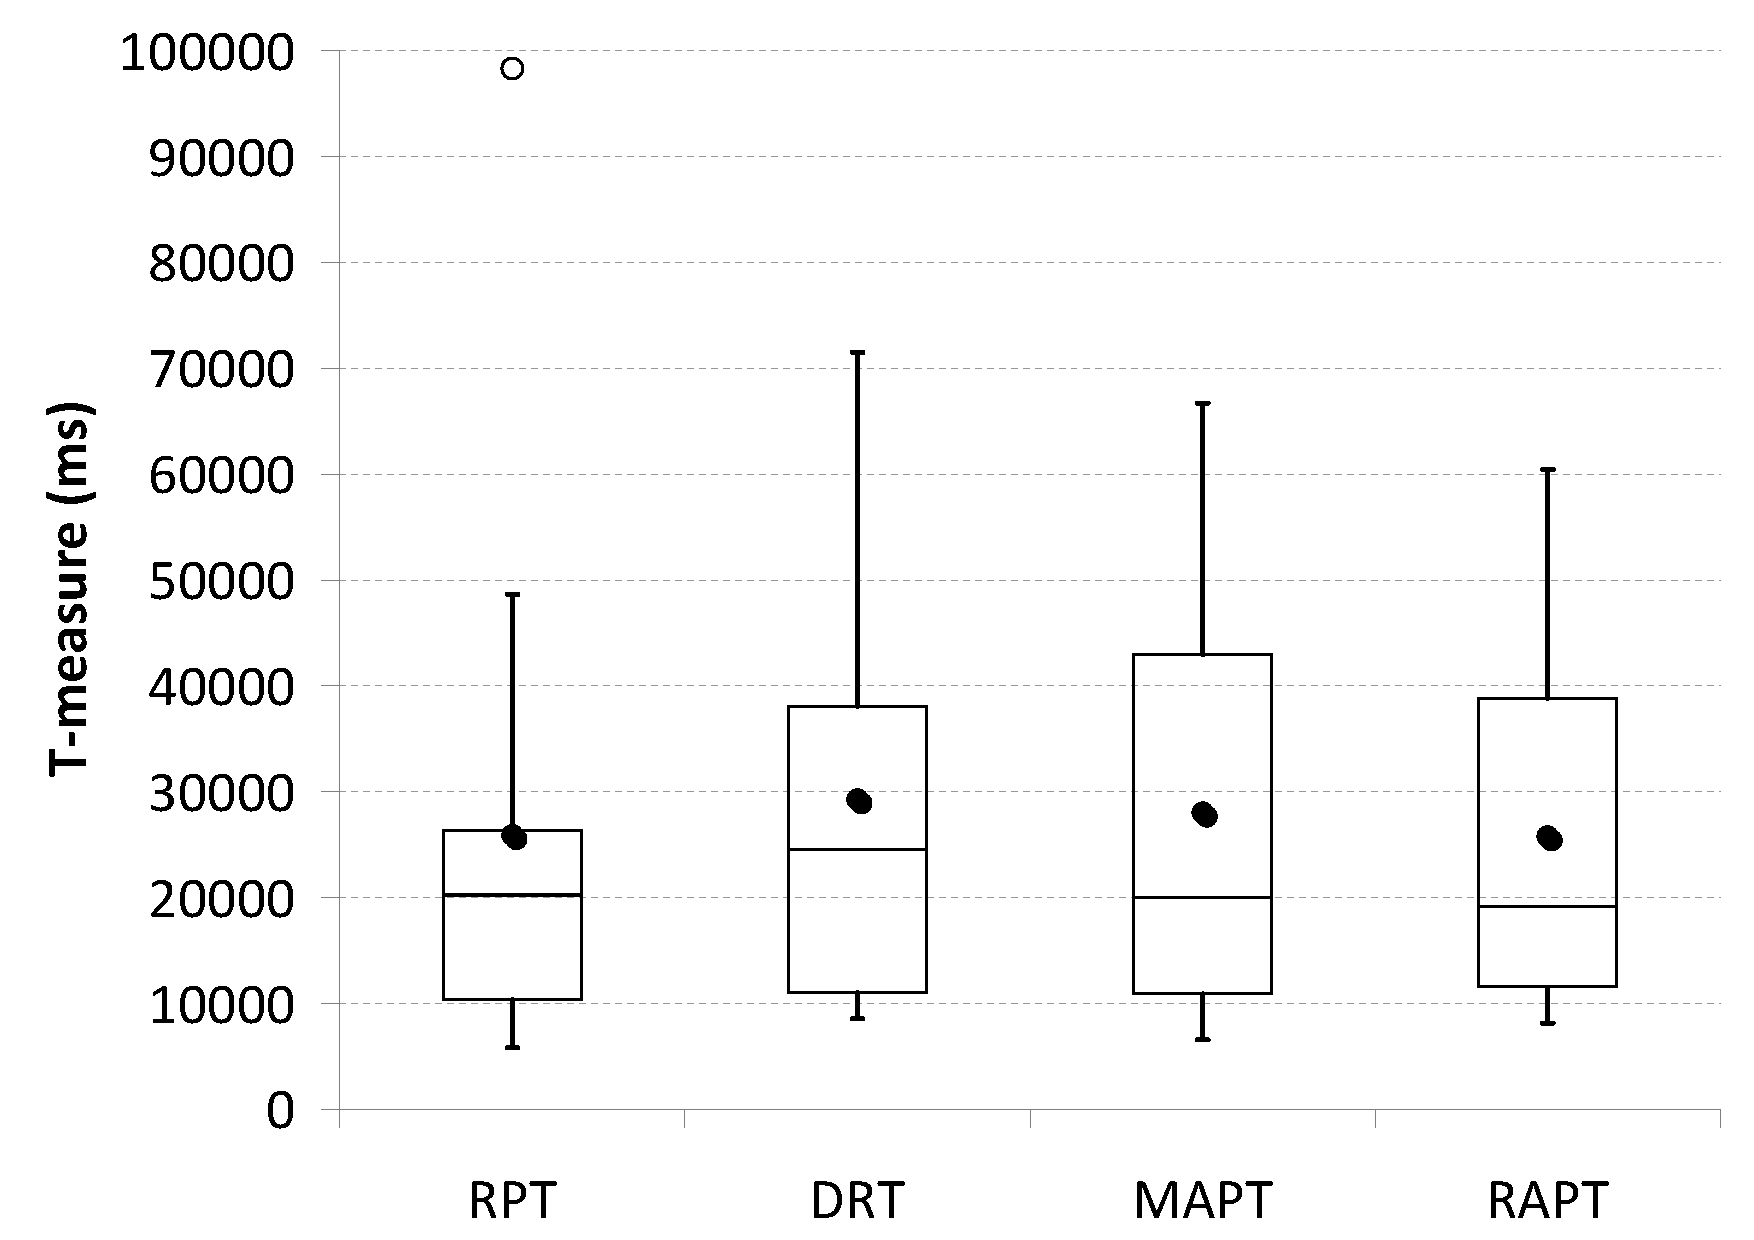
\includegraphics[width=0.32\textwidth]{makeT}}
%	\caption{Boxplots of T-measures on each object program}
%	\label{fig:Tmeasure}
%\end{figure*}
%
%\begin{figure*}[tp]
%	\centering
%	\subfigure[grep] {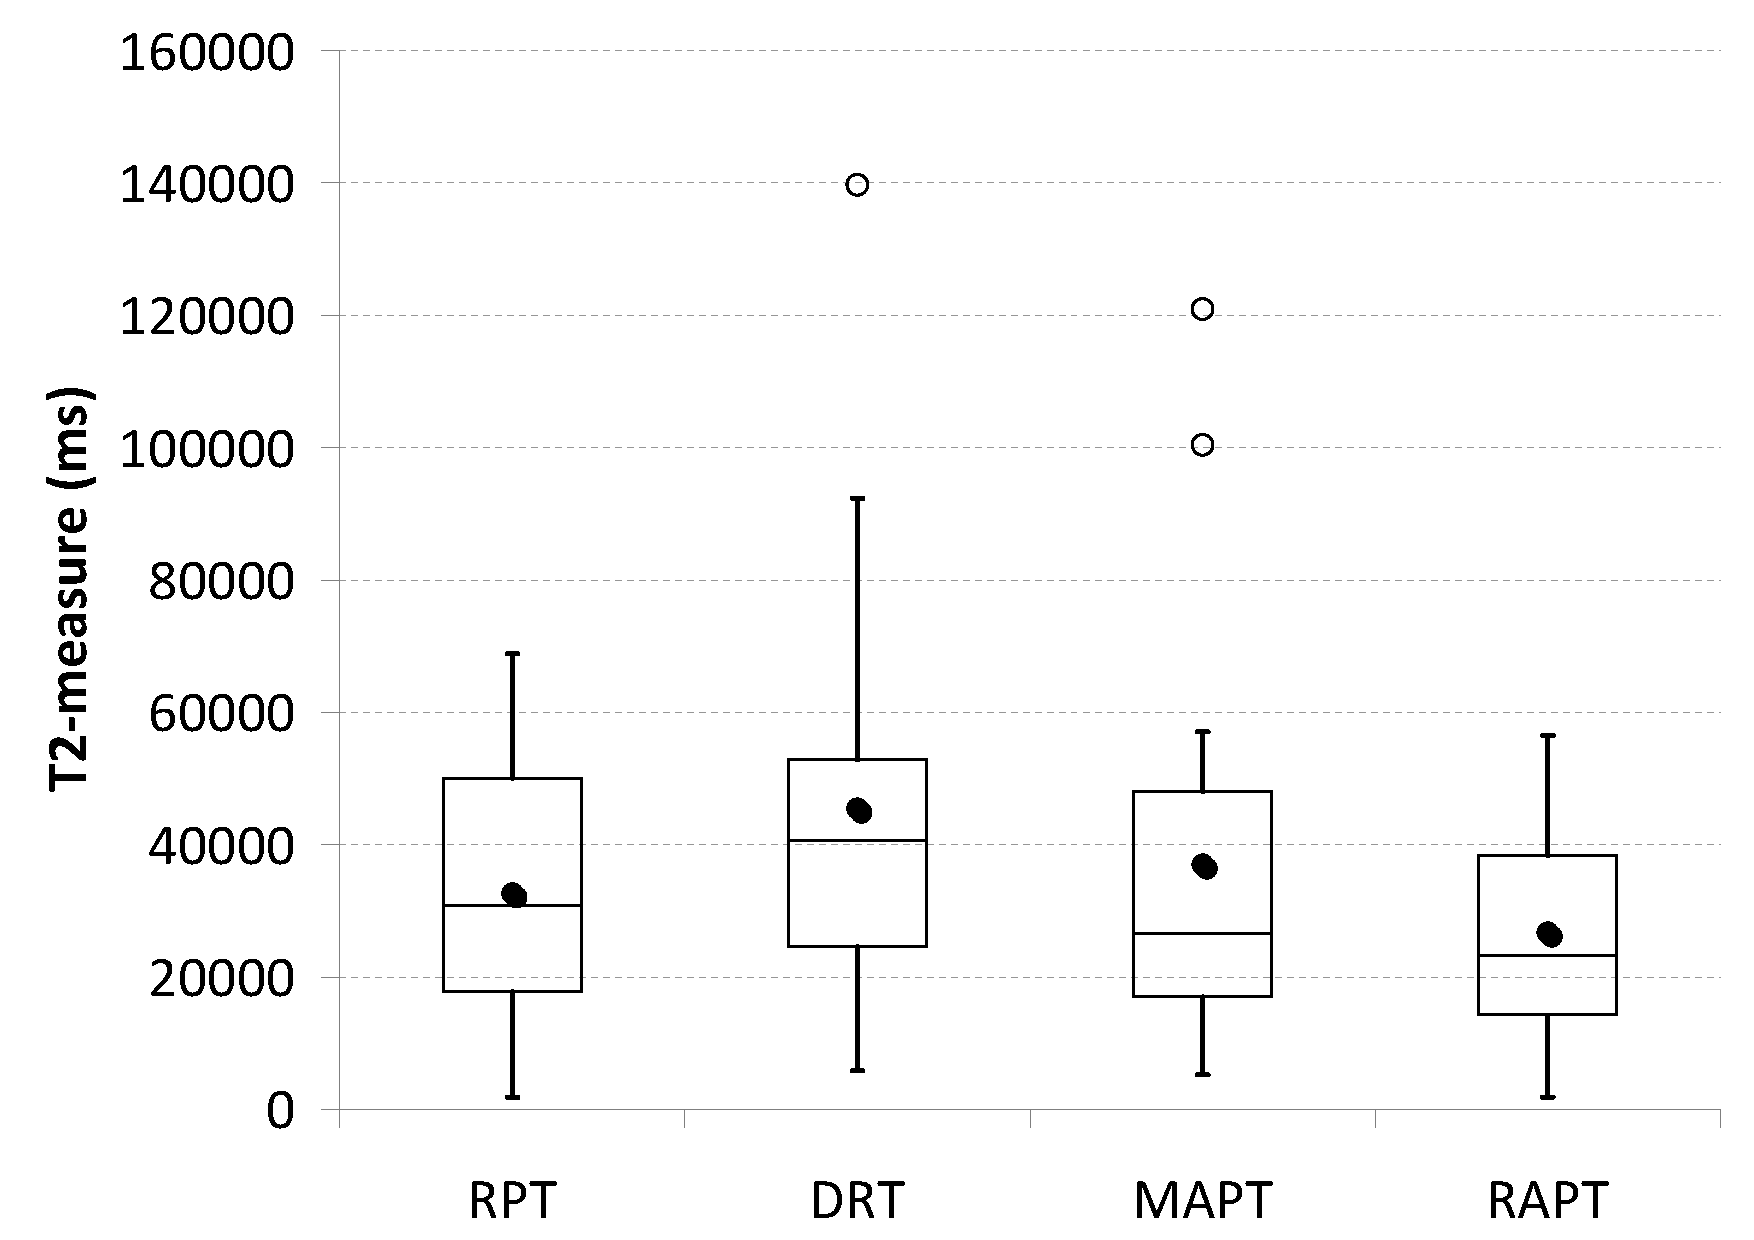
\includegraphics[width=0.32\textwidth]{grepT2}}
%    \subfigure[gzip] {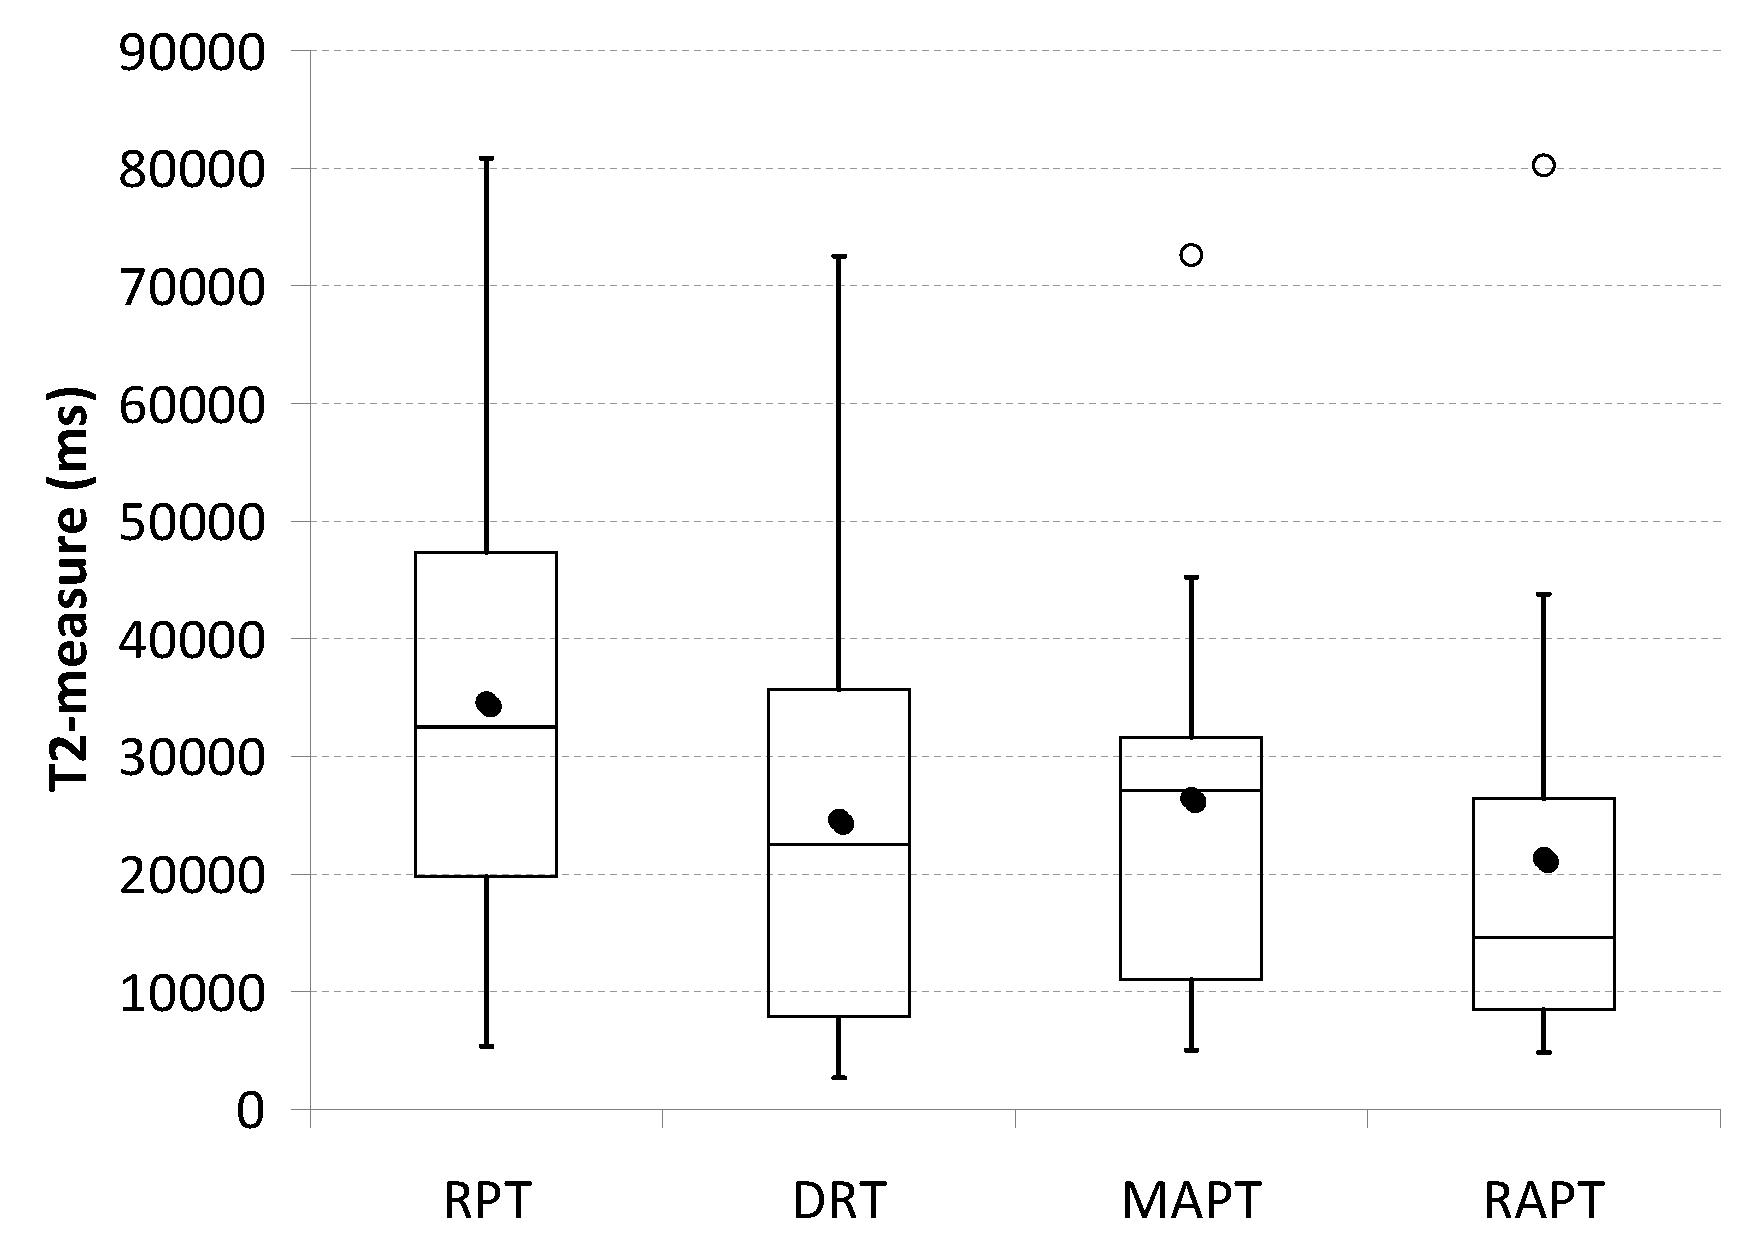
\includegraphics[width=0.32\textwidth]{gzipT2}}
%    \subfigure[make] {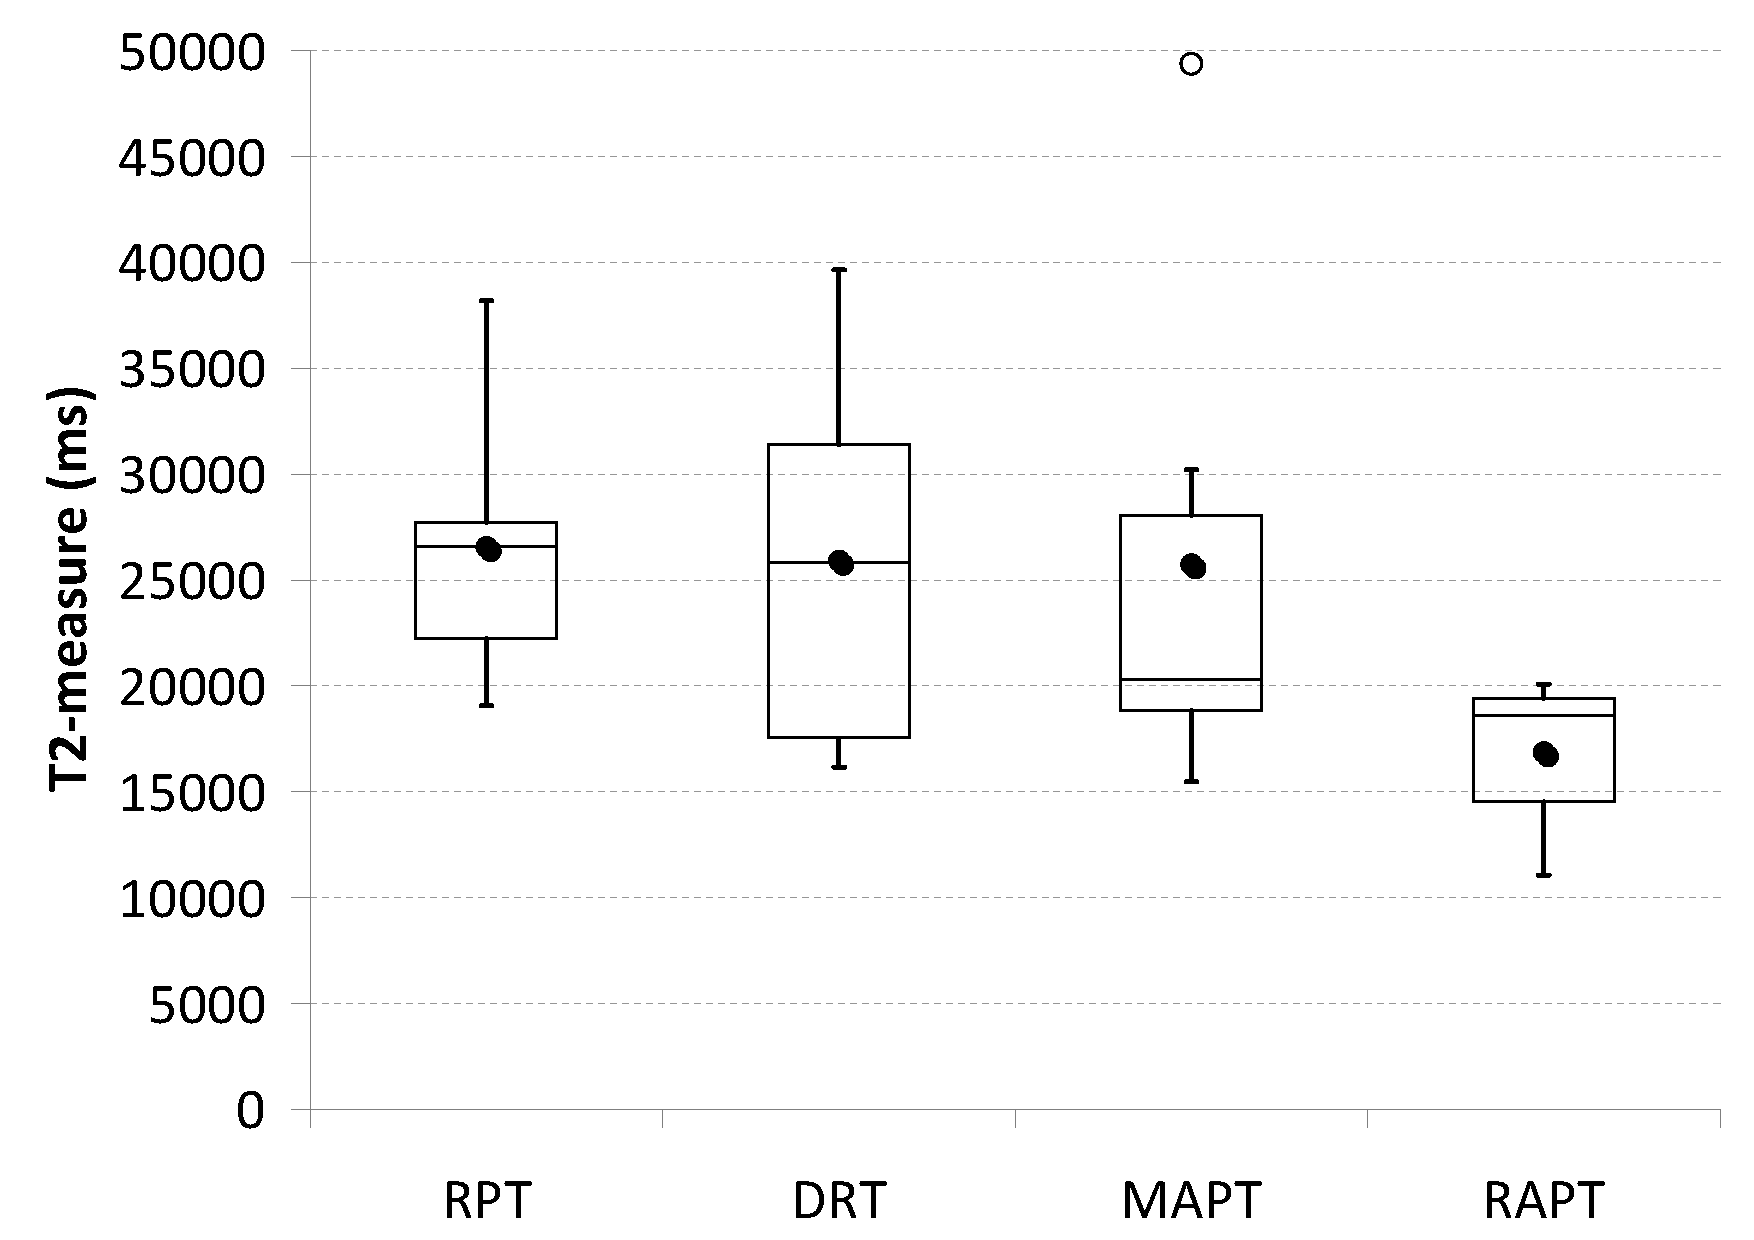
\includegraphics[width=0.32\textwidth]{makeT2}}
%	\caption{Boxplots of T2-measures on each object program}
%	\label{fig:T2measure}
%\end{figure*}
%
%We also used the Holm-Bonferroni method to determine which pair of testing techniques have significant difference in terms of T-measure and T2-measure, as shown in Tables~\ref{tab:Tsta} and~\ref{tab:T2sta}.
%
%\begin{table}
%\caption{Number of scenarios where the technique on top row has smaller T-measure than that on left column}
%\label{tab:Tsta}
%\centering
%\begin{tabular}{|c|c|c|c|c|} \hline
%			& RPT					& DRT					& MAPT				& RAPT				\\ \hline
%RPT		& ---					& 30					& 36					& \textbf{41}	\\ \hline
%DRT		& 30					& ---					& 36					& \textbf{41}	\\ \hline
%MAPT	& 24					& 24					& ---					& \textbf{39}	\\ \hline
%RAPT	& \textbf{19}	& \textbf{19}	& \textbf{21}	& ---					\\ \hline
%\end{tabular}
%\end{table}
%
%\begin{table}
%\caption{Number of scenarios where the technique on top row has smaller T2-measure than that on left column}
%\label{tab:T2sta}
%\centering
%\begin{tabular}{|c|c|c|c|c|} \hline
%			& RPT					& DRT					& MAPT				& RAPT				\\ \hline
%RPT		& ---					& 24					& \textbf{30}	& \textbf{33}	\\ \hline
%DRT		& 18					& ---					& 22					& \textbf{29}	\\ \hline
%MAPT	& \textbf{12}	& 20					& ---					& \textbf{32}	\\ \hline
%RAPT	& \textbf{9}	& \textbf{13}	& \textbf{10}	& ---					\\ \hline
%\end{tabular}
%\end{table}
%
%From Tables~\ref{tab:Tsta}, we can observe that in terms of T-measure, the performances of DRT and RPT were not distinguishable, and MAPT only marginally outperformed DRT and RPT. In addition, the performance of RAPT was significantly better than that of the other three techniques. Similar observation was made on the results of T2-measure, except that MAPT had significantly better T2-measure than RPT (whereas the T-measure difference between these two was marginal).
%%RAPT was significantly better than RPT.
%
%In summary, RAPT was consistently the best testing technique across all four metrics. MAPT was significantly better than DRT and RPT in terms of F-measure and F2-measure, but its outperformance was only marginal in terms of T-measure.
%% and T2-measure.
%
%\subsection{Further discussion}
%
%In our experiments, we have used three levels of granularity for partitioning as well as two types of initial probability profiles. We conducted further investigations to see whether there exist some strong correlations between the granularity/profile and the performance of APT.
%
%\subsubsection{Effect of granularity in partitioning}
%
%We compared each pair of granularity levels and conducted the statistical analysis on the comparison based on the Holm-Bonferroni method. The comparison results are summarized in Tables~\ref{tab:GstaF} to~\ref{tab:GstaT2}. In most cases, the effects of different granularity level on APT's performance were not significantly different. In other words, we could not observe a strong correlation between the granularity level in partitioning and the performance of APT.
%
%%As discussed in Section~\ref{sec:intro}, the key issue for a partitioning scheme is to ensure that each partition is homogeneous. However, no matter how coarse/fine the partitioning is, it is extremely difficult, if not impossible, to guarantee the homogeneity of every partition, especially considering that the faults are always unknown prior to testing. It is therefore uneasy to predict the fault-detection effectiveness by simply looking at the partitioning scheme and its granularity.
%
%\begin{table}
%\caption{Number of scenarios where the granularity level on top row is associated with smaller F-measure than that on left column}
%\label{tab:GstaF}
%\centering
%\begin{tabular}{|c|c|c|c|} \hline
%				& Coarse			& Medium			& Fine				\\ \hline
%Coarse	& ---					& 36					& 32					\\ \hline
%Medium	& 44					& ---					& \textbf{28}	\\ \hline
%Fine		& 48					& \textbf{52}	& ---					\\ \hline
%\end{tabular}
%\end{table}
%
%\begin{table}
%\caption{Number of scenarios where the granularity level on top row is associated with smaller F2-measure than that on left column}
%\label{tab:GstaF2}
%\centering
%\begin{tabular}{|c|c|c|c|} \hline
%				& Coarse			& Medium			& Fine				\\ \hline
%Coarse	& ---					& 25					& 19					\\ \hline
%Medium	& 31					& ---					& \textbf{17}	\\ \hline
%Fine		& 37					& \textbf{39}	& ---					\\ \hline
%\end{tabular}
%\end{table}
%
%\begin{table}
%\caption{Number of scenarios where the granularity level on top row is associated with smaller T-measure than that on left column}
%\label{tab:GstaT}
%\centering
%\begin{tabular}{|c|c|c|c|} \hline
%				& Coarse			& Medium			& Fine				\\ \hline
%Coarse	& ---					& 32					& \textbf{27}	\\ \hline
%Medium	& 48					& ---					& 33					\\ \hline
%Fine		& \textbf{53}	& 47					& ---					\\ \hline
%\end{tabular}
%\end{table}
%
%\begin{table}
%\caption{Number of scenarios where the granularity level on top row is associated with smaller T2-measure than that on left column}
%\label{tab:GstaT2}
%\centering
%\begin{tabular}{|c|c|c|c|} \hline
%				& Coarse			& Medium			& Fine				\\ \hline
%Coarse	& ---					& 29					& 21					\\ \hline
%Medium	& 27					& ---					& 19					\\ \hline
%Fine		& 35					& 37					& ---					\\ \hline
%\end{tabular}
%\end{table}
%
%\subsubsection{Effect of initial probability profile}
%
%We also compared the equal and proportional initial probability profiles in terms of their associated performance metrics. The comparison results are summarized in Table~\ref{tab:PstaF} to~\ref{tab:PstaT2}. It was shown that the proportional initial probability profile was significantly better than the equal one in terms of F2-measure, but the ranking was reversed when considering the T-measure. With respect to F-measure and T2-measure, there was no significant difference between these two types of initial probability profiles. In a word, we could not observe a strong correlation between the probability profile type and APT's performance.
%
%%Chen et al.~\cite{Chen01} demonstrated that if the number of test cases selected from each partition is proportional to the partition's size, PT should have a high fault-detection effectiveness. Our observation looks contradictory to this theory. However, it should be noted that the ``proportional'' profile in our experiments were designed according to the existing test suite, which was downloaded from SIR. It may not be truly proportional to the real size of each partition. In addition, since the identification of categories and choices in CPM is a subjective process, it is very difficult to fully avoid bias to provide a profile that is purely uniform.
%
%\begin{table}
%\caption{Number of scenarios where the initial profile type on top row is associated with smaller F-measure than that on left column}
%\label{tab:PstaF}
%\centering
%\begin{tabular}{|c|c|c|c|} \hline
%							& Equal				& Proportional	\\ \hline
%Equal					& ---					& 67						\\ \hline
%Proportional	& 53					& ---						\\ \hline
%\end{tabular}
%\end{table}
%
%\begin{table}
%\caption{Number of scenarios where the initial profile type on top row is associated with smaller F2-measure than that on left column}
%\label{tab:PstaF2}
%\centering
%\begin{tabular}{|c|c|c|c|} \hline
%							& Equal				& Proportional	\\ \hline
%Equal					& ---					& \textbf{28}		\\ \hline
%Proportional	& \textbf{56}	& ---						\\ \hline
%\end{tabular}
%\end{table}
%
%\begin{table}
%\caption{Number of scenarios where the initial profile type on top row is associated with smaller T-measure than that on left column}
%\label{tab:PstaT}
%\centering
%\begin{tabular}{|c|c|c|c|} \hline
%							& Equal				& Proportional	\\ \hline
%Equal					& ---					& \textbf{91}		\\ \hline
%Proportional	& \textbf{29}	& ---						\\ \hline
%\end{tabular}
%\end{table}
%
%\begin{table}
%\caption{Number of scenarios where the initial profile type on top row is associated with smaller T2-measure than that on left column}
%\label{tab:PstaT2}
%\centering
%\begin{tabular}{|c|c|c|c|} \hline
%							& Equal				& Proportional	\\ \hline
%Equal					& ---					& 51						\\ \hline
%Proportional	& 33					& ---						\\ \hline
%\end{tabular}
%\end{table}
%
%\section{Related Work}
%\label{sec:related}
%
%In this section, we will discuss the related work from the following four perspectives: (1) the integration of RT and PT, (2) the hypothesis of similarity among neighboring inputs, (3) the dynamic adjustment of test profile, and (4) the different treatments of fault-revealing and non-fault-revealing test cases.
%
%It is not a new idea to integrate RT and PT. RPT~\cite{Cai05, Cai07} may be the most straightforward technique for the integration, which selects a partition according to a pre-defined probability profile and selects test case from the partition. Cai~\cite{Cai02} also proposed adaptive testing (AT) based on the concept of software cybernetics. Lv et al.~\cite{LvTSE14} proposed an efficient AT strategy named Adaptive Testing with Gradient Descent method (AT-GD). Although AT outperformed both RT and PT in terms of fault-detection effectiveness, it requires very long execution time in reality. To address this efficiency problem, Lv et al.~\cite{Lv14} proposed a hybrid approach that uses AT and random partition testing (RPT) in an alternating manner. Furthermore, Cai et al.~\cite{Cai09} proposed DRT, where the probability profile is dynamically adjusted according to the testing information. DRT has been applied into others fields such as Web services~\cite{Sun12}. However, DRT makes use of fixed constants ($\epsilon$ and $\delta$) in the adjustment. Some studies~\cite{Lv11, Yang14, Li15} have been conducted to investigate the appropriate values for $\epsilon$ and $\delta$. However, the setting of these values may vary with different types of software. Compared with these techniques, our APT approach applies the novel mechanisms, such as MAPT and RAPT, to adaptively adjust the probability profile according to a variety of factors, which, in turn, are dynamically updated along the testing process.
%
%The proposal of APT is inspired by the common observation that fault-revealing inputs tend to cluster into continuous regions inside the input domain~\cite{White80, Ammann88, Finelli91, Bishop93, Koru08}. Adaptive random testing (ART)~\cite{Chen10}, a family of enhance RT techniques, is also based on this observation. The basic notion of ART is ``even spread'': Because of the similarity of neighboring inputs, it is better to select a test case that is far away from the previous non-fault-revealing test cases. Compared with APT, ART mainly focus on enhancing the effectiveness of RT by evenly spreading test cases across the input domain; in other words, it does not consider PT. Recently, CPM was used to help improve the applicability of ART into programs with non-numeric inputs~\cite{Barus16} --- the concepts of categories and choices were applied to provide a metric for measuring the dissimilarity between non-numeric test cases.
%%The partitioning component of CPM was not applied in ART. In a word, although
%APT and ART are based on the same hypothesis of similar behavior for neighboring inputs, but they attempt to improve the testing effectiveness from different perspectives.
%
%There exist other studies that also involve the dynamic adjustment of test profile. Chen et al.~\cite{Chen09}, for example, proposed that the test profile should be dynamically revised according to the distribution of previously executed test cases. Similar work was further conducted by Liu et al.~\cite{Liu11}, where dynamic test profiles were designed to simulate various ART algorithms. The profiles investigated in these studies are actually the probability distribution of concrete test cases, while the profile in APT is the distribution for partitions.
%
%One key issue of APT (and DRT) is that the profile will be adjusted in almost opposite ways depending on whether or not a test case reveals a fault. Such an arrangement is understandable because fault-revealing and non-fault-revealing test cases shall deliver quite different information. However, this issue was unfortunately not considered in some techniques. For instance, quasi-random testing~\cite{Chen07, Liu16} attempts to achieve the even spread of test cases by leveraging the features of low discrepancy and low dispersion of quasi-random sequences. Its test case selection process is not affected by the fault detection information at all. Liu et al.~\cite{Liu12} studied the influence of fault-revealing test cases on the performance of ART, and found that if the fault-revealing test case was completely ``forgotten'' when selecting the next test case, ART would have better effectiveness in detecting multiple faults. Apparently, such a forgetting strategy is somewhat naive and not as fine-grained as the profile adjustment mechanisms used in MAPT and RAPT. In addition, Zhou et al.~\cite{Zhou09} proposed a technique to select test cases based on the online fault-detection information: The fault-revealing test cases will have high probability to be selected for the testing. This technique actually adjusted the selection of concrete test cases, while the adjustment mechanisms in our APT approach are conducted on the selection of partition that contains the next test case.
%
%\section{Conclusion}
%\label{sec:conc}
%
%RT and PT are two fundamental families of software testing techniques. Each of them has its own merit and weakness, and sometimes they can be complementary to each other. Some studies have been conducted to integrate RT and PT, resulting in some advanced testing techniques, such as RPT and DRT. In this paper, we proposed a new approach to integrating RT and PT, namely APT. In APT, a test profile is maintained and adaptively updated based on some novel mechanisms, including the Markov matrix (MAPT) and the reward and punishment strategy (RAPT). Empirical studies have been conducted to evaluate the performance of MAPT and RAPT using three large-sized real-life programs associated with ten faulty versions and 19 distinct faults. It has shown that both RAPT and MAPT can use significantly fewer test cases than DRT and RPT. We have also observed that RAPT has significantly lower overhead than DRT and RPT, while MAPT's overhead is only marginally lower than that of DRT and RPT.
%
%Our experiments involved three levels of granularity and two types of initial probability profile. Our investigations showed that there was no strong correlation between the granularity/profile and the performance. It is thus necessary to further study the proper partitioning scheme(s) with appropriate granularity level for APT and relevant techniques. It is also of importance to investigate how to design a ``good'' probability profile aiming at optimizing the testing effectiveness.
%
%One piece of future work is about the appropriate settings of the parameters (such as $\epsilon$, $\delta$, $\gamma$, and $\tau$) in APT. The settings we used in this study are based on the previous experience and/or empirical estimation. It is worthwhile to investigate the relationship between different settings and the performance of APT, and thus hopefully work out a guideline on how to set these parameters. Our empirical studies compared APT with two baseline techniques that integrate RT and PT. It is also interesting to further compare APT with other testing techniques, such as ART. Last but not the least, it is possible to integrate MAPT and RAPT as well as other relevant techniques, with the purpose of further enhancing the performance of APT.
%
%%\appendices
%%\section{Proof of the First Zonklar Equation}
%%Appendix one text goes here.
%
%% use section* for acknowledgment
%\ifCLASSOPTIONcompsoc
%  % The Computer Society usually uses the plural form
%  \section*{Acknowledgments}
%\else
%  % regular IEEE prefers the singular form
%  \section*{Acknowledgment}
%\fi
%
%
%This research is supported by the National Natural Science Foundation of China under Grant No. 61370061, the Beijing Natural Science Foundation (Grant No. 4162040), the Beijing Municipal Training Program for Excellent Talents under Grant No.2012D009006000002, and the Aeronautical Science Foundation of China (Grant No. 2016ZD74004).
%
%
%
%% can use a bibliography generated by BibTeX as a .bbl file
%% BibTeX documentation can be easily obtained at:
%% http://mirror.ctan.org/biblio/bibtex/contrib/doc/
%% The IEEEtran BibTeX style support page is at:
%% http://www.michaelshell.org/tex/ieeetran/bibtex/
%\bibliographystyle{IEEEtran}
%% argument is your BibTeX string definitions and bibliography database(s)
%\bibliography{APT}
%%
%
%
%
%
%% Can use something like this to put references on a page
%% by themselves when using endfloat and the captionsoff option.
%\ifCLASSOPTIONcaptionsoff
%  \newpage
%\fi


% that's all folks
\end{document}


